\let\negmedspace\undefined
\let\negthickspace\undefined
\documentclass[journal]{IEEEtran}
\usepackage[a5paper, margin=10mm, onecolumn]{geometry}

\usepackage{tfrupee}
\usepackage{tipa}
\usepackage{graphicx} % Required for inserting images
\usepackage{amsmath,amsthm,amssymb,amsfonts}
\usepackage{multicol}
\usepackage[utf8]{inputenc}
\usepackage{titling}
\usepackage{geometry}[margin=1.5cm]
\usepackage{gvv-book}
\usepackage{gvv}
\usepackage{cite}
\usepackage{amsmath,amssymb,amsfonts,amsthm}
\usepackage{algorithmic}
\usepackage{graphicx}
\usepackage{textcomp}
\usepackage{xcolor}
\usepackage{txfonts}
\usepackage{listings}
\usepackage{enumitem}
\usepackage{mathtools}
\usepackage{gensymb}
\usepackage{comment}
\usepackage[breaklinks=true]{hyperref}
\usepackage{tkz-euclide} 
\usepackage{listings}                                        
\def\inputGnumericTable{}                                 
\usepackage[latin1]{inputenc}                                
\usepackage{color}                                            
\usepackage{array}                                            
\usepackage{longtable}                                       
\usepackage{calc}                                             
\usepackage{multirow}                                         
\usepackage{hhline}                                           
\usepackage{ifthen}                                           
\usepackage{lscape}

\setlength{\droptitle}{-1cm}
\title{\textbf{XH - 2022}}
\author{EE25BTECH11050 - Hema Havil}
\begin{document}
\maketitle
\section*{\large \underline{\textbf {GATE 2022 General Aptitude (GA)}}}
\vspace{0.2cm}
\subsection*{\underline{\textbf{Q.1-Q.5 Carry ONE mark each}}}

\begin{enumerate}

\item Inhaling the smoke from a burning could you quickly.
\begin{multicols}{2}
\begin{enumerate}[label=(\Alph*)]
\item tire/tier
\item tire/tyre
\item tyre/tire
\item tyre/tier
\end{enumerate}
\end{multicols}
\hfill\textbf{(GATE-XH-2022)}

\item A sphere of radius r cm is packed in a box of cubical shape. What should be the minimum volume (in cm$^3$) of the box that can enclose the sphere?
\begin{multicols}{2}
\begin{enumerate}
\item $\frac{r^{3}}{8}$
\item $r^{3}$
\item $2r^{3}$
\item $8r^{3}$
\end{enumerate}
\end{multicols}
\hfill\textbf{(GATE-XH-2022)}

\item Pipes P and Q can fill a storage tank in full with water in 10 and 6 minutes, respectively. Pipe R draws the water out from the storage tank at a rate of 34 litres per minute. P, Q and R operate at a constant rate. If it takes one hour to completely empty a full storage tank with all the pipes operating simultaneously, what is the capacity of the storage tank (in litres)?
\begin{multicols}{2}
\begin{enumerate}
\item 26.8
\item 60.0
\item 120.0
\item 127.5
\end{enumerate}
\end{multicols}
\hfill\textbf{(GATE-XH-2022)}

\item Six persons P, Q, R, S, T and U are sitting around a circular table facing the center not necessarily in the same order. Consider the following statements: P sits next to S and T. Q sits diametrically opposite to P. The shortest distance between S and R is equal to the shortest distance between T and U. Based on the above statements, Q is a neighbor of
\begin{enumerate}
\begin{multicols}{2}
\item U and S
\item R and T
\item R and U
\item P and S
\end{multicols}
\end{enumerate}
\hfill\textbf{(GATE-XH-2022)}

\item A building has several rooms and doors as shown in the top view of the building given below. The doors are closed initially. What is the minimum number of doors that need to be opened in order to go from the point P to the point Q?
\begin{figure}[h!]
\centering
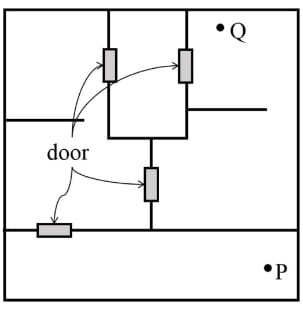
\includegraphics[width=0.5\columnwidth]{figs/Q5.jpg}
\caption*{}
\label{fig:placeholder}
\end{figure}
\begin{enumerate}
\begin{multicols}{4}
\item 4
\item 3
\item 2
\item 1
\end{multicols}
\end{enumerate}
\hfill\textbf{(GATE-XH-2022)}
\subsection*{ \underline{ \textbf{Q.6-Q.10 Carry TWO marks each}}}
\vspace{0.3cm}

\item Rice, a versatile and inexpensive source of carbohydrate, is a critical component of diet worldwide. Climate change, causing extreme weather, poses a threat to sustained availability of rice. Scientists are working on developing Green Super Rice (GSR), which is resilient under extreme weather conditions yet gives higher yields sustainably. Which one of the following is the CORRECT logical inference based on the information given in the above passage?
\begin{enumerate}
\item GSR is an alternative to regular rice, but it grows only in an extreme weather
\item GSR may be used in future in response to adverse effects of climate change
\item GSR grows in an extreme weather, but the quantity of produce is lesser than regular rice
\item Regular rice will continue to provide good yields even in extreme weather
\end{enumerate}
\hfill\textbf{(GATE-XH-2022)}

\item A game consists of spinning an arrow around a stationary disk as shown below. When the arrow comes to rest, there are eight equally likely outcomes. It could come to rest in any one of the sectors numbered 1, 2, 3, 4, 5, 6, 7 or 8 as shown. Two such disks are used in a game where their arrows are independently spun. What is the probability that the sum of the numbers on the resulting sectors upon spinning the two disks is equal to 8 after the arrows come to rest?
\begin{figure}[h!]
\centering
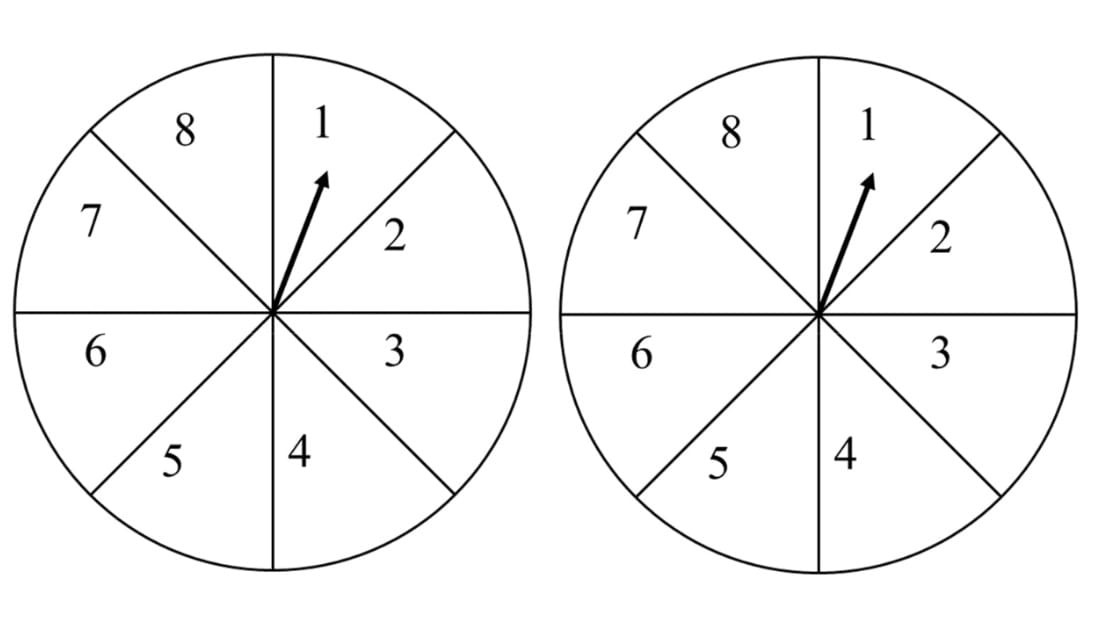
\includegraphics[width=0.5\columnwidth]{figs/Q7.jpg}
\caption*{}
\label{fig:placeholder}
\end{figure}
\begin{multicols}{4}
\begin{enumerate}
\item $\frac{1}{16}$
\item $\frac{5}{64}$
\item $\frac{3}{32}$
\item $\frac{7}{64}$
\end{enumerate}
\end{multicols}
\hfill\textbf{(GATE-XH-2022)}

\item Consider the following inequalities. $3p-q<4$ (i) $3q-p<12$ (ii) Which one of the following expressions below satisfies the above two inequalities?
\begin{multicols}{4}
\begin{enumerate}
\item $p+q<8$
\item $p+q=8$
\item $8\le p+q<16$
\item $p+q\ge16$
\end{enumerate}
\end{multicols}
\hfill\textbf{(GATE-XH-2022)}

\item Given below are three statements and four conclusions drawn based on the statements. Statement 1: Some engineers are writers. Statement 2: No writer is an actor. Statement 3: All actors are engineers. Conclusion I: Some writers are engineers. Conclusion II: All engineers are actors. Conclusion III: No actor is a writer. Conclusion IV: Some actors are writers. Which one of the following options can be logically inferred?
\begin{enumerate}
\item Only conclusion I is correct
\item Only conclusion II and conclusion III are correct
\item Only conclusion I and conclusion III are correct
\item Either conclusion III or conclusion IV is correct
\end{enumerate}
\hfill\textbf{(GATE-XH-2022)}

\item Which one of the following sets of pieces can be assembled to form a square with a single round hole near the center? Pieces cannot overlap.
\begin{enumerate}
\item 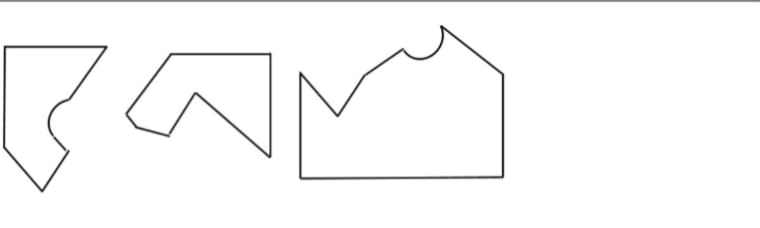
\includegraphics[width=0.5\columnwidth]{figs/Q10(A).jpeg}
\item 
\includegraphics[width=0.5\columnwidth]{figs/Q10(B).jpg}
\item 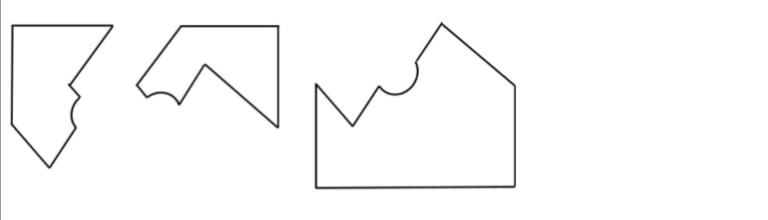
\includegraphics[width=0.5\columnwidth]{figs/Q10(C).jpeg}
\item 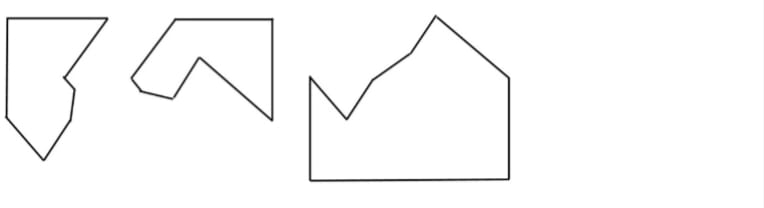
\includegraphics[width=0.5\columnwidth]{figs/Q10(D).jpeg}

\end{enumerate}
\hfill\textbf{(GATE-XH-2022)}
\newpage
\section*{\large \underline{\textbf {GATE 2022 Humanities and Social Sciences - Economics (XH-C1)}}}
\vspace{0.2cm}
\subsection*{ \underline{\textbf {XH-B1: Q.11 – Q.17 Carry ONE mark Each}}}

\item A relationship is expressed as Iodine: Goitre. The pair(s) of words showing SIMILAR relationship is/are
\begin{enumerate}
\item Mango: Anaemia
\item Insulin: Diabetes
\item Fat: Obesity
\item Hormones: Heredity
\end{enumerate}
\hfill\textbf{(GATE-XH-2022)}

\item Three individuals are named P, Q, and R. Together they have a total of fifteen children of which nine are boys. P has three girls and Q has same number of boys. Q has one more child than P, who has four children. R has four more boys than the number of girls. The number of girls of R is equal to the number of boys of P. How many boys do R and P have?
\begin{multicols}{4}
\begin{enumerate}
\item $R=3$ $P=3$
\item $R=4$ $P=2$
\item $R=5$, $P=1$
\item $R=2$, $P=4$
\end{enumerate}
\end{multicols}
\hfill\textbf{(GATE-XH-2022)}

\item A sentence has been given below. The train will leave at 8:30 PM, we have been ready by 7:30 PM, so that we can reach the station on time. To make the above sentence grammatically correct, the phrase marked in bold is to be replaced by
\begin{enumerate}
\item were
\item are
\item must be
\item should have
\end{enumerate}
\hfill\textbf{(GATE-XH-2022)}

\item Complete the sentence correctly using the options given below. Hastings\underline{\hspace{1cm}}$(p)$\underline{\hspace{1cm}} developed as a holiday resort after \underline{\hspace{1cm}}$(q)$\underline{\hspace{1cm}} .
\begin{enumerate}
\item $(p)$ = a seaside town, $(q)$ = the first world war
\item $(p)$ = , a seaside town, $(q)$ = the First World War
\item $(p)$ = , a Seaside Town, $(q)$ = World War I
\item $(p)$ = A seaside town $(q)$ = World War I
\end{enumerate}
\hfill\textbf{(GATE-XH-2022)}

\item The Arecibo telescope does not resemble what most of us think of when we hear the word telescope. Its reflective surface covers an area of 20 acres, which is quite remarkable. Dangling above it are towers and cables, sub-reflectors and antennas, all of which can be positioned using 26 motors to transmit radio waves and receive echoes with astonishing precision. From the passage, it can be inferred that most telescopes
\begin{enumerate}
\item are not as large as Arecibo
\item do not have reflective surface
\item cannot be re-positioned
\item strictly have 26 motors
\end{enumerate}
\hfill\textbf{(GATE-XH-2022)}

\item Tailgating another vehicle is unsafe and illegal. Many rear-end collisions are caused by drivers following too close to the vehicle in front of them. The rules state that a driver must keep significant distance from the vehicle in front in order to stop safely and avoid a collision. Drivers should allow a minimum two seconds gap between their vehicle and the one ahead. At 60 km per hour, this equates to a gap of 33 meters; at 100 km per hour, it equates to a gap of 55 meters. More distance is needed to safely stop in rain or poor visibility, as during rain slippery roads reduce the effectiveness of braking. Which of the following statement(s) can be inferred from the above passage?
\begin{enumerate}
\item People drive faster in rain and under poor visibility.
\item Braking may not be as effective during rain as in the dry conditions.
\item Tailgating is against the road rules.
\item Collision has no relationship with tailgating.
\end{enumerate}
\hfill\textbf{(GATE-XH-2022)}

\item There are three separate, but equal-sized boxes. Inside each box, there are two separate small boxes. Inside each of the small boxes, there are four even smaller boxes. The total number of boxes will be \underline{\hspace{3cm}} .
\hfill\textbf{(GATE-XH-2022)}
\vspace{0.2cm}
\subsection*{\underline{\textbf {Q.18 – Q.26 Carry TWO marks Each}}}

\item In a specific language, xer dan means ``big horse'', liro cas means ``red tomato'' and dum cas dan means ``big red barn''. The equivalent word for barn in this language is
\begin{enumerate}
\item dum
\item liro
\item dan
\item cas
\end{enumerate}
\hfill\textbf{(GATE-XH-2022)}

\item Park street is parallel to Rock street. Garden street is perpendicular ($90^\circ$) to Lake street. Lake street is parallel to Rock street. For the situation described above, the TRUE statement is
\begin{enumerate}
\item Park street is perpendicular to Lake street
\item Rock street is parallel to Garden street
\item Park street is parallel to Garden street
\item Garden street is perpendicular to Park street
\end{enumerate}
\hfill\textbf{(GATE-XH-2022)}

\item Six examinations are required to be conducted in a week starting from Sunday to Saturday. Hindi is not scheduled on the first day and English is not scheduled before Hindi. Mathematics is scheduled one day after Physics. Biology is scheduled two days after Hindi. One day prior to Chemistry, there is no examination. Only one examination can be scheduled on a single day and Sunday is not an off day. What are the subjects scheduled on first and the last days?
\begin{enumerate}
\item First day Physics, Last day Biology
\item First day Physics, Last day Chemistry
\item First day Physics, Last day English
\item First day English, Last day Biology
\end{enumerate}
\hfill\textbf{(GATE-XH-2022)}

\item A passage consists of 6 sentences. The first and sixth sentences of the passage are at their correct positions, while the middle four sentences (represented by P, Q, R, and S) are jumbled up. First sentence: Smoke oozed up between the planks. P: Passengers were told to be ready to quit the ship. Q: The rising gale fanned the smouldering fire. R: Everyone now knew there was fire onboard. S: Flames broke out here and there. Sixth sentence: Most people bore the shock bravely. The most logically CORRECT order for the given jumbled up sentences is
\begin{enumerate}
\item QSRP
\item QPSR
\item RSPQ
\item PQRS
\end{enumerate}
\hfill\textbf{(GATE-XH-2022)}
\item For a painting to succeed, it is essential that the painter and his public agree about what is significant. The subject of the painting may have a personal meaning for the painter or a common person; but there can also be the possibility of their agreement on its general meaning. It is at this point that the culture of the society and the period in question precedes the artists and her/his art. Renaissance art would have meant nothing to the Aztecs, and vice versa. If, to some extent, a few intellectuals can appreciate them both today, it is because their culture is a historical one. Its inspiration is history and all known developments to date.

According to the passage, which of the following is/are NOT necessarily among the attributes needed for a painter to succeed?

\begin{enumerate}
\item The subject must have a personal meaning for the painter.
\item The painter is able to communicate and justify the significance of its subject selection.
\item The painter and the public agree on what is significant.
\item The painting of the subjects is driven by public demand.
\end{enumerate}
\hfill\textbf{(GATE-XH-2022)}
\item Vinod has a pre-determined route. Each morning he delivers 37 newspapers to customers in his neighborhood. It takes Vinod 50 minutes to deliver all the papers. When Vinod was sick or had other engagements, his friend Tarun, who lives on the same street delivered the papers on his behalf.

Find the statement(s) that must be TRUE according to the given information.

\begin{enumerate}
\item Vinod and Tarun lived in the same locality.
\item It was dark outside when Vinod began his delivery.
\item It took Tarun more than 50 minutes to deliver the papers.
\item Tarun delivered 37 newspapers to customers.
\end{enumerate}
\hfill\textbf{(GATE-XH-2022)}
\item Cholera, typhoid, diphtheria and tuberculosis cause huge number of deaths. Poor quality drinking water has always been the world’s greatest single carrier of sickness. Disease is transmitted when sewage and drinking water come into contact. Children are particularly vulnerable. In some of the poorest countries the infant mortality rate is high. The separation of sewage and the supply of clean drinking water are the domain of civil engineers, and their work makes a significant contribution to public health. That contribution was recognized when public sanitation was voted the greatest medical breakthrough, beating the discoveries including antibiotics and vaccines in a poll organized by the British Medical Journal.

Identify the statement(s), which is/are NOT TRUE according to the passage.

\begin{enumerate}
\item Children are less prone to water borne diseases.
\item The infant mortality rate was high in economically weaker countries.
\item The provision of sewage and drinking water should be adequately separated from each other.
\item The literature states that the public health and sanitation was never given its due importance.
\end{enumerate}
\hfill\textbf{(GATE-XH-2022)}
\item Shark’s teeth have evolved to correspond to the diet of each particular species of shark. Consequently, the teeth of the great white shark bear little resemblance to those of the bull shark or nurse shark. There were essentially four different shark diets and thus four varieties of shark teeth. Sharks that feed on fish have needle like teeth, perfect for spearing and ripping. Sharks that eat mammals such as seals and sea lions have heavy, serrated teeth, typically triangular on the upper jaw and pointed on the lower jaw. Shark that feed in the benthic zone of the ocean have flattened teeth for crushing the shell of the creatures they find scuttling in the sand or clinging to rocks. Sharks that bask have teeth that are largely non-functional; these sharks filter food from the water by passing it through their gills.

Which of the following is/are the CORRECT inference(s) as per the passage?

\begin{enumerate}
\item Shark’s teeth are not specially designed for slaughter.
\item The shape of the shark’s teeth relates to its prey.
\item Some species of sharks filter food through their gills.
\item Shark’s teeth relate to its diet.
\end{enumerate}
\hfill\textbf{(GATE-XH-2022)}

\item A particular school management wants to contact all parents, all businessmen and all engineers. The following statistics are available with the school.\\
Businessmen = 50\\
Engineers = 25\\
Parents = 2500\\
Businessmen who are engineers = 0\\
Businessmen who are parents = 25\\
Engineers who are parents = 15\\
The number of people needs to be contacted are \underline{\hspace{2cm}}
\hfill\textbf{(GATE-XH-2022)}
\subsection*{\underline{\textbf { XH-C1 (Q.27 – Q.44 Carry ONE mark Each)}}}
\item Suppose that a firm has a technology represented by the following production function:\\
\begin{equation*}
   {Y(K,L)=K^x L^y}
\end{equation*}
  where K denotes capital, L denotes labour, Y denotes the maximum output that is possible to produce using capital K and labour L. \textit{x} and \textit{y} are two positive real numbers. It is also known that the production function satisfies constant returns to scale. Then which of the following is true?
\begin{enumerate}
\item x+y=0.5
\item x+y=1
\item x+y=1.5
\item x+y=2
\end{enumerate}
\hfill\textbf{(GATE-XH-2022)}
\item The Human Development Index (HDI), as reported by the United Nations Development Program, is based on three components. Two of these components are per-capita income and a measure of educational attainment of society. The third component is
\begin{enumerate}
\item Gini coefficient
\item percentage of population who have access to safe drinking water
\item percentage of population who work in non-agricultural sector
\item life expectancy at birth
\end{enumerate}
\hfill\textbf{(GATE-XH-2022)}

\item Suppose we estimate the following regression equation:
\begin{equation*}
    ln(x_t)=\alpha_0 +\alpha_1ln(y_t)\quad \alpha_0,\alpha_1>0
\end{equation*}
where $x_t$ and $y_t$ are some variables. $\alpha_0$ and $\alpha_1$ are the intercept and the slope,
respectively. $\epsilon_t$ is the residual term. What is the interpretation of the coefficient $\alpha_1$?
\begin{enumerate}
\item A 1\% increase in $y_t$ causes a $\alpha_1$\% increase in $x_t$
 
\item A 1\% increase in $y_t$ causes a $\alpha_1$ ×0.01 unit increase in $x_t$
 
\item A one unit increase in $y_t$ causes a 100×$\alpha_1$ \% increase in $x_t$
 
\item A one unit increase in $y_t$ causes a  $\alpha_1$ unit increase in $x_t$
 
\end{enumerate}
\hfill\textbf{(GATE-XH-2022)}
\item Consider the following system of equations in three variables x,y,z:\\
\begin{equation*}
    -x-y-z=3
\end{equation*}
\begin{equation*}
    x+y+z=10
\end{equation*}
\begin{equation*}
    2x-3y=6
\end{equation*}

This system of equations has
\begin{enumerate}
\item no combination of values of $(x,y,z)$ that satisfy this system simultaneously
\item only one combination of values of $(x,y,z)$ that satisfy this system simultaneously
\item only two combinations of values of $(x,y,z)$ that satisfy this system simultaneously
\item infinitely many combinations of values of $(x,y,z)$ that satisfy this system simultaneously
\end{enumerate}
\hfill\textbf{(GATE-XH-2022)}

\item Which of the following models appropriately explains the fluctuations in potential output and long-run aggregate supply by understanding the shocks to productivity or the willingness of the worker?
\begin{multicols}{2}
\begin{enumerate}
\item Solow growth model
\item Real business cycle model
\item IS-LM model
\item Harrod-Domar Model
\end{enumerate}
\end{multicols}
\hfill\textbf{(GATE-XH-2022)}

\item The change in equilibrium output for an equal amount of change in government expenditure and tax revenue is linked to which one of the following multipliers?
\begin{multicols}{2}
\begin{enumerate}
\item Expenditure multiplier
\item Balanced Budget multiplier
\item Lum-sum tax multiplier
\item Trade multiplier
\end{enumerate}
\end{multicols}
\hfill\textbf{(GATE-XH-2022)}

\item Solaris is a firm that can install solar panels at an airport to generate electricity for the airport’s usage. The company claims that in 70 percent of all airports where its solar panels are installed, an airport’s electricity bill is reduced by at least 40 percent. The probability that an airport’s electricity bill is reduced by at least 40 percent, in seven out of ten airports where the company’s solar panels are installed, equals approximately:
\begin{multicols}{2}
\begin{enumerate}
\item 0.082
\item 0.002
\item 0.490
\item 0.267
\end{enumerate}
\end{multicols}
\hfill\textbf{(GATE-XH-2022)}

\item IndiaSMart is a retail shop that accepts either a Rupay credit card, or a Visa credit card. 31 percent of IndiaSMart’s customers carry a Rupay credit card, 44 percent of its customers carry a Visa credit card, while 18 percent of its customers carry a Rupay credit card as well as a Visa credit card. What is the probability that a customer carries at least one of the two, i.e. either a Rupay or a Visa credit card?
\begin{multicols}{2}
\begin{enumerate}
\item 0.75
\item 0.93
\item 0.57
\item 0.49
\end{enumerate}
\end{multicols}
\hfill\textbf{(GATE-XH-2022)}

\item What is the user cost of capital for a firm when the rate of depreciation of machine is 20\% and the cost of financial capital is 15\%?
\begin{multicols}{2}
\begin{enumerate}
\item 37\%
\item 50\%
\item 35\%
\item 31\%
\end{enumerate}
\end{multicols}
\hfill\textbf{(GATE-XH-2022)}

\item Which among the following Gini coefficients exhibits the highest equality?
\begin{multicols}{2}
\begin{enumerate}
\item 0.1
\item 0.2
\item 0.5
\item 0.6
\end{enumerate}
\end{multicols}
\hfill\textbf{(GATE-XH-2022)}

\item Let $f(x, y)$ be a continuously differentiable homogenous function of degree 4. Which of the following is necessarily true?
\begin{multicols}{2}
\begin{enumerate}
\item $\displaystyle x \frac{\partial f(x, y)}{\partial x} + y \frac{\partial f(x, y)}{\partial y} = f(x, y)$
\item $\displaystyle x \frac{\partial f(x, y)}{\partial x} + y \frac{\partial f(x, y)}{\partial y} = 2f(x, y)$
\item $\displaystyle x \frac{\partial f(x, y)}{\partial x} + y \frac{\partial f(x, y)}{\partial y} = 4f(x, y)$
\item $\displaystyle x \frac{\partial f(x, y)}{\partial x} + y \frac{\partial f(x, y)}{\partial y} = 8f(x, y)$
\end{enumerate}
\end{multicols}
\hfill\textbf{(GATE-XH-2022)}

\item Which of the following committees was set-up to address issues related to capital account convertibility in India?
\begin{multicols}{2}
\begin{enumerate}
\item Tandon Committee
\item Abid Hussain Committee
\item Tarapore Committee
\item Percy Mistry Committee
\end{enumerate}
\end{multicols}
\hfill\textbf{(GATE-XH-2022)}

\item The demand curve for tea in Borduria is given by
\[
D(P) = 40-2P
\]
and the domestic supply curve of tea in Borduria is given by
\[
S(P) = P
\]
Here $D(P)$ denotes quantity demanded when price is $P$ and $S(P)$ is quantity supplied by domestic producers at price $P$. Tea is traded in a competitive world market and imported into Borduria at a price of 9 per unit. Initially there was no restriction on trade. However, as a result of lobbying by the domestic suppliers, the Bordurian government imposes a tariff of 3 per unit on each unit imported. As a result of the tariff, import of tea decreased by how many units?
\begin{multicols}{4}
\begin{enumerate}
\item 2
\item 3
\item 8
\item 9
\end{enumerate}
\end{multicols}
\hfill\textbf{(GATE-XH-2022)}
\item Bretton Woods agreement gave birth to the following organization:
\begin{multicols}{2}
\begin{enumerate}
\item GATT
\item RBI
\item NAFTA
\item ASEAN
\end{enumerate}
\end{multicols}
\hfill\textbf{(GATE-XH-2022)}

\item Which one of the following is a test of heteroscedastity?
\begin{multicols}{2}
\begin{enumerate}
\item White test
\item Jarque-Bera test
\item Breusch-Godfrey test
\item Ljung-box test
\end{enumerate}
\end{multicols}
\hfill\textbf{(GATE-XH-2022)}

\item The law that explains the relationship between income growth and the size of government expenditure is appropriately linked to:
\begin{multicols}{2}
\begin{enumerate}
\item Wagner’s law
\item Okun’s law
\item Walras law
\item Ricardian equivalence
\end{enumerate}
\end{multicols}
\hfill\textbf{(GATE-XH-2022)}

\item As per recent Economic Survey, how many states and Union Territories (UTs) are driven by services sector in India?
\begin{multicols}{2}
\begin{enumerate}
\item 15
\item 19
\item 25
\item 21
\end{enumerate}
\end{multicols}
\hfill\textbf{(GATE-XH-2022)}

\item An economy is characterized by the following production function:
\[
Y = A K^{0.25} L^{0.75}
\]
where $K$ denotes capital, $L$ denotes labour, $A$ denotes the total factor productivity and $Y$ denotes output produced. All capital and labour are fully employed. Suppose that the growth rate of labour is $1\%$, the growth rate of capital is $4\%$, and the growth rate of output is $4\%$. The growth rate of total factor productivity $A$ is:
\begin{multicols}{4}
\begin{enumerate}
\item 1.5\%
\item 1.75\%
\item 2.25\%
\item 2.5\%
\end{enumerate}
\end{multicols}
\hfill\textbf{(GATE-XH-2022)}
\subsection*{\underline{\textbf{Q.45 – Q.65 Carry TWO marks Each}}}

\item Suppose a firm has the following production function:
\[
f(x_1, x_2, x_3, x_4) = \min\{x_1, x_2\} + \min\{x_3, x_4\}
\]
The per unit cost of input $x_i$ is given by $w_i$, where $i = 1, 2, 3, 4$. Suppose that $w_1 = 1$, $w_2 = 5$, $w_3 = 3$, and $w_4 = 6$. If the firm is minimizing cost, which of the following input choices by the firm can be observed?
\begin{multicols}{2}
\begin{enumerate}
\item $x_1 > 0, x_2 = 0, x_3 > 0, x_4 = 0$
\item $x_1 > 0, x_2 > 0, x_3 = 0, x_4 = 0$
\item $x_1 > 0, x_2 = 0, x_3 = 0, x_4 > 0$
\item $x_1 = 0, x_2 = 0, x_3 > 0, x_4 > 0$
\end{enumerate}
\end{multicols}
\hfill\textbf{(GATE-XH-2022)}
\item Suppose an econometrician had specified the following regression:
\[
y = \beta_0 + \beta_1 z_1 + \beta_2 z_2 + \beta_3 z_3 + \epsilon
\]
but a researcher estimated the following regression:
\[
y = \beta_0 + \beta_1 z_1 + \beta_2 z_2 + \beta_3 z_3 + \beta_4 z_4 + \epsilon
\]
What will be the consequence of including the irrelevant variable on the estimated coefficients?
\begin{enumerate}
\item Coefficient estimates will be unbiased, consistent but inefficient
\item Coefficient estimates will be consistent, asymptotically efficient but biased
\item Coefficient estimates will be inconsistent and efficient
\item Coefficient estimates will be biased, consistent and efficient
\end{enumerate}
\hfill\textbf{(GATE-XH-2022)}

\item Okun’s law says that a 1\% increase in unemployment for one year is associated with a 2\% decrease in GDP growth. Suppose an economy has the following expectations augmented Phillips curve:
\[
\pi = \pi^e - \beta(U - U^n), \quad \beta > 0
\]
where $\pi$ and $\pi^e$ are the inflation and expected inflation rates, respectively, $U$ and $U^n$ are the unemployment and natural rate of unemployment, respectively. $\beta$ measures sensitivity of inflation to unemployment gap. When $\beta = 2$, by what percentage does output fall short of full-employment given that the inflation rate, expected inflation rate and natural rate of unemployment are 8\%, 10\% and 6\%, respectively?
\begin{multicols}{4}
\begin{enumerate}
\item 2
\item 4
\item 6
\item 8
\end{enumerate}
\end{multicols}
\hfill\textbf{(GATE-XH-2022)}

\item Let $f(x)$ be the probability distribution function of a random variable $X$, where
\[
f(x) = \frac{5x^4}{64}, \quad -2 < x < 2
\]
and $f(x) = 0$ otherwise. Let $|\cdot|$ denote the modulus function. Then, $P(|X| < 1)$ and $P(X^2 < 3)$ are given by (respectively):
\begin{multicols}{4}
\begin{enumerate}
\item $\frac{1}{32}$ and $\frac{9\sqrt{3}}{32}$
\item $\frac{5}{64}$ and $\frac{5\sqrt{3}}{32}$
\item $\frac{1}{64}$ and $\frac{\sqrt{3}}{32}$
\item $\frac{2\sqrt{3}}{32}$ and $\frac{1}{32}$
\end{enumerate}
\end{multicols}
\hfill\textbf{(GATE-XH-2022)}

\item Liquidity Adjustment Facility (LAF) uses the following instruments:
\begin{enumerate}
\item Call Money Rate and Mumbai Inter-bank Offered Rate
\item Repo Rate and Reverse Repo Rate
\item Bank Rate and Statutory Liquidity Ratio
\item Cash Reserve Ratio and Prime Lending Rate
\end{enumerate}
\hfill\textbf{(GATE-XH-2022)}
\item What is the weightage of manufacturing sector in the Index of Industrial Production (IIP) during 2020-2021?  

Note: numbers are in approximate values  
\begin{multicols}{2}
\begin{enumerate}
\item 78\%
\item 81\%
\item 65\%
\item 71\%
\end{enumerate}
\end{multicols}
\hfill\textbf{(GATE-XH-2022)}

\item The curve that explains the relationship between tax rate and tax revenue is known as:
\begin{multicols}{2}
\begin{enumerate}
\item Laffer curve
\item Engle curve
\item Beveridge curve
\item Phillips curve
\end{enumerate}
\end{multicols}
\hfill\textbf{(GATE-XH-2022)}

\item Suppose the estimated consumption equation of an economy is:
\[
C = 40 + \beta Y
\]
where $Y$ is the personal disposable income, $\beta$ is the marginal propensity to consume (MPC). Government expenditure ($G$) is given as 90. Total tax ($T$) received is $\delta Y$, where $Y$ is aggregate output or real income and $\delta$ is tax to real income proportionality factor. Autonomous investment ($I$) is given as 80. What are the tax revenue and budget surplus of the government when $\beta = 0.75$ and $\delta = 0.20$? All units are measured in constant rupees.
\begin{enumerate}
\item Tax revenue = Rs. 105 and surplus = Rs. 15
\item Tax revenue = Rs. 118 and surplus = Rs. 28
\item Tax revenue = Rs. 110 and surplus = Rs. 20
\item Tax revenue = Rs. 125 and surplus = Rs. 35
\end{enumerate}
\hfill\textbf{(GATE-XH-2022)}

\item Consider a two-period consumption model in which a representative household lives for two periods only. In period 1, he earns income $y_1$ and consumes $c_1$. In period 2, he earns $y_2$ and consumes $c_2$. He can borrow and lend at the same rate of interest ($r$). His lifetime utility function is as follows:
\[
U(c_1, c_2) = \ln(c_1) + \beta \ln(c_2)
\]
where $\beta > 0$ measures the sensitivity of future period’s consumption. What will be the marginal propensity to consume of current consumption?
\begin{multicols}{4}
\begin{enumerate}
\item $\frac{1}{1+\beta}$
\item $\frac{\beta}{1+\beta}$
\item $\frac{y}{1+\beta}$
\item $\frac{1}{2(1+\beta)} y$
\end{enumerate}
\end{multicols}
\hfill\textbf{(GATE-XH-2022)}

\item Suppose an investigator has specified the following simultaneous equation model:
\[
y_{1,t} = \alpha_{1,0} + \alpha_{1,1} y_{1,t-1} + \alpha_{1,2} M_t + \alpha_{1,3} K_t + u_t \tag{1}
\]
\[
y_{2,t} = \alpha_{2,0} + \alpha_{2,1} y_{1,t} + \alpha_{2,3} I_t + \nu_t \tag{2}
\]
where $y_{1,t}$ and $y_{2,t}$ are endogenous variables, $M_t$, $K_t$, and $I_t$ are predetermined variables, and $u_t$ and $\nu_t$ are residual terms. Based on the order condition of identification, which one of the following statements are correct?
\begin{enumerate}
\item Equations (1) and (2) are exactly identified
\item Equation (1) is exactly identified and equation (2) is over-identified
\item Equation (1) is over-identified and equation (2) is exactly identified
\item Both the equations are under-identified
\end{enumerate}
\hfill\textbf{(GATE-XH-2022)}

\item There are two regions in a country. The demand for chocolates in region 1 is given by
\[
Q_1(P) = 100 - P
\]
and the demand for chocolates in region 2 is given by
\[
Q_2(P) = 200 - P
\]
where $Q_1(P)$ and $Q_2(P)$ denote the demand for chocolates in region 1 and 2 respectively at a price $P$. There is only one seller who is licensed to sell chocolates in the country. Suppose the seller sets a price of $P = 125$. The total demand for chocolates in the country at this price is:
\begin{multicols}{4}
\begin{enumerate}
\item 50
\item 75
\item 100
\item 125
\end{enumerate}
\end{multicols}
\hfill\textbf{(GATE-XH-2022)}

\item A producer manufactures batteries by using techniques I and II. The capacities (in ampere hours) of 12 randomly selected batteries manufactured by using technique I are: 140, 132, 136, 142, 138, 150, 154, 150, 152, 136, 144 and 142. Moreover, the capacities (in ampere hours) of 14 randomly selected batteries manufactured by using technique II are: 144, 134, 132, 130, 136, 146, 140, 128, 131, 128, 150, 137, 130 and 135.\\
Suppose that battery capacities manufactured by using techniques I and II are normally distributed, with unknown means, $\mu_I$ and $\mu_{II}$ respectively, and an unknown common variance $\sigma^2$. Consider the null hypothesis $H_0: (\mu_I - \mu_{II}) = \gamma$ ampere hours.  

For which of the following values of $\gamma$ should the null hypothesis $H_0$ be accepted, against the alternative hypothesis $H_1: (\mu_I - \mu_{II}) \neq \gamma$ ampere hours, at 10\% level of significance?
\begin{multicols}{4}
\begin{enumerate}
\item $\gamma = 4$
\item $\gamma = 7$
\item $\gamma = 10$
\item $\gamma = 13$
\end{enumerate}
\end{multicols}
\hfill\textbf{(GATE-XH-2022)}

\item Tom and Jerry both arrive at a petrol pump. Without worrying about price, Tom says, “I want 10 liters of petrol.” Also, without worrying about price, Jerry says, “I want petrol worth 1000 rupees.” The own price elasticities of demand for Tom (denoted by $\epsilon_T$) and Jerry (denoted by $\epsilon_J$) are:
\begin{multicols}{2}
\begin{enumerate}
\item $\epsilon_T = 0, \ \epsilon_J = -\infty$
\item $\epsilon_T = 0, \ \epsilon_J = -1$
\item $\epsilon_T = -\infty, \ \epsilon_J = 0$
\item $\epsilon_T = -1, \ \epsilon_J = 0$
\end{enumerate}
\end{multicols}
\hfill\textbf{(GATE-XH-2022)}

\item Which of the following variables are pushed upwards by ‘Seigniorage’?
\begin{multicols}{2}
\begin{enumerate}
\item Money supply
\item Inflation
\item Tax rate
\item Interest rate
\end{enumerate}
\end{multicols}
\hfill\textbf{(GATE-XH-2022)}

\item Suppose Raju enters the job market at age 25 and earns annual income of Rs. 6000. He retires at age 65 and his life expectancy is 75 years. He does not own any assets. Assume that Raju consumes annual income uniformly over his lifetime. What will be his average propensity to consume during employment years?
\begin{multicols}{4}
\begin{enumerate}
\item 0.90
\item 0.80
\item 0.50
\item 0.40
\end{enumerate}
\end{multicols}
\hfill\textbf{(GATE-XH-2022)}
\item A monopolist faces the following inverse demand function:
\[
P = 40 - Q,
\]
where $P$ denotes price and $Q$ denotes quantity. The monopolist has zero fixed cost and a marginal cost of 5 per unit of output produced. The monopolist aims to maximize profit. Suppose the government imposes a tax of 5 per unit of output on the monopolist. As a result, the price charged by the profit-maximizing monopolist to the consumer increases by:
\begin{multicols}{4}
\begin{enumerate}
\item 0
\item 2.5
\item 5
\item 10
\end{enumerate}
\end{multicols}
\hfill\textbf{(GATE-XH-2022)}

\item In the flexible exchange rate environment with perfect capital mobility, a fiscal stimulus will be linked to which of the following statements?
\begin{enumerate}
\item Fiscal policy increases the domestic outcome
\item Fiscal policy does not increase the domestic output
\item Fiscal policy leads domestic exports to fall
\item Fiscal policy appreciates the domestic currency
\end{enumerate}
\hfill\textbf{(GATE-XH-2022)}

\item Consider a lottery with two possible outcomes:
\begin{itemize}
    \item Rupees 100 with probability 0.6  
    \item  Rupees 50 with probability 0.4  
\end{itemize}    
The maximum amount that a risk-neutral person would be willing to pay to play the above lottery equals Rupees \underline{\hspace{2cm}} (in integer).
\hfill\textbf{(GATE-XH-2022)}
\vspace{0.2cm}

\item Mr. Sharma’s consumption preference for tea (denoted by $x$) and sugar (denoted by $y$) is given by the utility function  
\[
U(x, y) = \min\{x, 2y\}
\]
The price per unit of tea is 10 and the price per unit of sugar is 10. Mr. Sharma’s total income is 900. The optimum quantity of tea purchased by Mr. Sharma equals \underline{\hspace{2cm}} (in integer).
\hfill\textbf{(GATE-XH-2022)}
\vspace{0.2cm}

\item Suppose $\alpha$ is a real number between 0 and 1. Rohit is choosing $x$ and $y$ to maximize the following utility function:\\  
{\center {$U(x, y) = x^2 + 2xy + y^2 + 4\alpha + 8\alpha^2 + 10$}}\\
subject to the following constraints:  
\[
2x + y = 10,\quad x, y \geq 0
\]
Then the optimal value of $y$ chosen by Rohit is \underline{\hspace{1cm}} (in integer). 
\hfill\textbf{(GATE-XH-2022)}
\vspace{0.2cm}

\item In a competitive market for dry-cleaning, the inverse market demand function is given by
\[
P = 100 - Q
\]
where $P$ denotes price and $Q$ denotes quantity. The (private) marginal cost (MC) of production for all the dry-cleaning firms together is given by
\[
MC = 20 + 2Q
\]
The market pollution generated by the dry-cleaning processes of all firms creates external damages given by the marginal external cost (MEC):
\[
MEC = 2Q
\]
The socially efficient output of dry-cleaning is \underline{\hspace{2cm}} (in integer).\\
\hfill\textbf{(GATE-XH-2022)}
\newpage
\section*{\large \underline{\textbf {GATE 2022 English (XH-C2)}}}
\subsection*{ \underline{\textbf {Q.66 – Q.83 Carry ONE mark each}}}

\item ``He who is unable to live in society, or who has no need because he is sufficient for himself, must be either a beast or a god.''  
Who has given the above statement?
\begin{multicols}{4}
\begin{enumerate}
\item Aristotle
\item Plato
\item Socrates
\item Rousseau
\end{enumerate}
\end{multicols}
\hfill\textbf{(GATE-XH-2022)}

\item ``History is not made only in statecraft; its lasting results are produced in the ranks of learned men.''  
Name the play from which the above excerpt has been taken.
\begin{enumerate}
\item Mahesh Dattani’s \textit{Thirty Days in September}
\item Vijay Tendulkar’s \textit{Silence! The Court is in Session}
\item Girish Karnad’s \textit{Tughlaq}
\item Rabindranath Tagore’s \textit{Mukta-Dhara}
\end{enumerate}
\hfill\textbf{(GATE-XH-2022)}

\item Who amongst the following popularised the term `objective correlative', which is often used in formalist criticism?
\begin{multicols}{2}
\begin{enumerate}
\item Virginia Woolf
\item C. S. Lewis
\item Matthew Arnold
\item T. S. Eliot
\end{enumerate}
\end{multicols}
\hfill\textbf{(GATE-XH-2022)}

\item Which of the following critics preferred Shakespeare’s comedies to his tragedies?
\begin{multicols}{2}
\begin{enumerate}
\item Samuel Johnson
\item Alexander Pope
\item John Dryden
\item Thomas De Quincey
\end{enumerate}
\end{multicols}
\hfill\textbf{(GATE-XH-2022)}

\item Who among the following has been credited with laying the foundation of comparative literature by Russian Formalists?
\begin{multicols}{2}
\begin{enumerate}
\item Viktor Shklovsky
\item Alexander Veselovsky
\item Vladimir Propp
\item Roman Jakobson
\end{enumerate}
\end{multicols}
\hfill\textbf{(GATE-XH-2022)}

\item \textit{Lyrical Ballads}, considered to be the manifesto of Romantic Poetry, was first published in the year \underline{\hspace{2cm}}.
\begin{multicols}{4}
\begin{enumerate}
\item 1795
\item 1797
\item 1789
\item 1798
\end{enumerate}
\end{multicols}
\hfill\textbf{(GATE-XH-2022)}

\item Identify the work from which the following excerpt has been taken:  
``In a universe that is suddenly deprived of illusions and of light, man feels a stranger. He is an irremediable exile …. This divorce between man and his life, the actor and his setting, truly constitutes the feeling of Absurdity.''
\begin{multicols}{2}
\begin{enumerate}
\item Franz Kafka’s \textit{The Trial}
\item Samuel Beckett’s \textit{Waiting for Godot}
\item Albert Camus’ \textit{The Myth of Sisyphus}
\item Harold Pinter’s \textit{The Homecoming}
\end{enumerate}
\end{multicols}
\hfill\textbf{(GATE-XH-2022)}

\item What does gynocriticism recommend as an approach to literature?
\begin{enumerate}
\item Considering women’s literature from men’s point of view
\item Examining women’s literature confirming gender stereotypes only
\item Becoming more familiar with the history of women and women’s writing
\item Becoming more familiar with gerontology
\end{enumerate}
\hfill\textbf{(GATE-XH-2022)}

\item Identify the novel which opens with the following lines:  
``It was the best of times, it was the worst of times, it was the age of wisdom, it was the age of foolishness, it was the epoch of belief, it was the epoch of incredulity, it was the season of light, it was the season of darkness, it was the spring of hope, it was the winter of despair.''
\begin{multicols}{2}
\begin{enumerate}
\item Jane Austen’s \textit{Emma}
\item Emily Brontë’s \textit{Wuthering Heights}
\item Charles Dickens’ \textit{A Tale of Two Cities}
\item H. G. Wells’ \textit{The Time Machine}
\end{enumerate}
\end{multicols}
\hfill\textbf{(GATE-XH-2022)}

\item Which of the following terms does not form a part of seven types of ambiguities propounded by William Empson?
\begin{multicols}{4}
\begin{enumerate}
\item Simulacra
\item Metaphor
\item Pun
\item Simile
\end{enumerate}
\end{multicols}
\hfill\textbf{(GATE-XH-2022)}

\item Which of the following poem(s) has/have been influenced by Hindu philosophy?
\begin{multicols}{2}
\begin{enumerate}
\item The Solitary Reaper
\item Brahma
\item The Curse of Kehama
\item Kubla Khan
\end{enumerate}
\end{multicols}
\hfill\textbf{(GATE-XH-2022)}

\item Which of the following human behaviour(s) is/are important to a Freudian psychoanalytical study of William Shakespeare’s \textit{Hamlet}?
\begin{multicols}{2}
\begin{enumerate}
\item Art of speaking
\item Changes in emotional states
\item Neurotic behaviour
\item Merry-making
\end{enumerate}
\end{multicols}
\hfill\textbf{(GATE-XH-2022)}

\item Which of the following novel-author combination(s) is/are correct?
\begin{enumerate}
\item \textit{Where Shall We Go This Summer} – Jane Austen
\item \textit{A Passage to England} – Nirad C. Chaudhuri
\item \textit{The Mayor of Casterbridge} – Thomas Hardy
\item \textit{Pride and Prejudice} – Anita Desai
\end{enumerate}
\hfill\textbf{(GATE-XH-2022)}

\item Which of the following statements is/are correct about Phenomenology?
\begin{enumerate}
\item It is a form of methodological idealism, seeking to explore an abstraction called `human consciousness'.
\item It is a philosophical method associated with Edmund Husserl.
\item It believes that the act of thinking and the object of thought are internally related, mutually dependent.
\item Heidegger’s \textit{Being and Time} is an important phenomenological treatise supporting the stand of Husserl.
\end{enumerate}
\hfill\textbf{(GATE-XH-2022)}

\item Chitra Divakaruni’s \textit{The Mistress of Spices} is \underline{\hspace{3cm}}.
\begin{multicols}{2}
\begin{enumerate}
\item an experiment in magic realism
\item about immigrant experience
\item a science fiction
\item an epistolary novel
\end{enumerate}
\end{multicols}
\hfill\textbf{(GATE-XH-2022)}

\item Which of the following is/are correct about postmodernist critics?
\begin{enumerate}
\item They foreground fiction and exemplify `disappearance of the real'.
\item They foreground irony.
\item They tend towards reflexivity.
\item They challenge the distinction between high and low cultures.
\end{enumerate}
\hfill\textbf{(GATE-XH-2022)}

\item The literary theory of Deconstruction argues that \underline{\hspace{3cm}}.
\begin{enumerate}
\item texts are always heterogeneous
\item the meaning of a text never relies on context
\item any system for the production of meaning may be bound by context, yet also limitless
\item texts are always rigid in meaning
\end{enumerate}
\hfill\textbf{(GATE-XH-2022)}

\item In the context of the Reader-Response Theory, Louise M. Rosenblatt in her essay ``The Poem as Event'', considers that the reader should \underline{\hspace{3cm}}.
\begin{enumerate}
\item participate in a transaction with the text
\item act against a text
\item be acted upon by the text
\item reject the text
\end{enumerate}
\hfill\textbf{(GATE-XH-2022)}
\subsection*{\underline{\textbf{Q.84 – Q.103 Carry TWO marks each.}}}

\item Roland Barthes in his famous essay, ``The Death of the Author'' \underline{\hspace{3cm}}.
\begin{enumerate}
\item believes that the text is to be interpreted in the biographical context of the author
\item challenges the author’s claim as ``cogito'', or origin of all knowledge
\item believes that the author has sole claim to his work
\item concludes that an author is an atypical product of his social milieu
\end{enumerate}
\hfill\textbf{(GATE-XH-2022)}

\item What is common among the following novels?  
Cormac McCarthy’s \textit{The Road}  
George Orwell’s \textit{Nineteen Eighty-Four}  
Margaret Atwood’s \textit{The Handmaid’s Tale}
\begin{multicols}{2}
\begin{enumerate}
\item They are utopian novels
\item They are dystopian novels
\item They are postmodern novels
\item They are war novels
\end{enumerate}
\end{multicols}
\hfill\textbf{(GATE-XH-2022)}

\item Which of the following is/are true about the ``New Historicism'' school of literary criticism?
\begin{enumerate}
\item It arose in the 1980s, influenced by the work of Michel Foucault.
\item It emphasizes the historical context of a text.
\item It regards literary and non-literary texts as equally important in understanding a cultural moment.
\item It treats history as a narrative subject to interpretation.
\end{enumerate}
\hfill\textbf{(GATE-XH-2022)}

\item Identify the author of the novel \textit{The Namesake}.
\begin{multicols}{2}
\begin{enumerate}
\item Jhumpa Lahiri
\item Arundhati Roy
\item Chitra Banerjee Divakaruni
\item Kiran Desai
\end{enumerate}
\end{multicols}
\hfill\textbf{(GATE-XH-2022)}

\item Which of the following novels is NOT by Salman Rushdie?
\begin{multicols}{2}
\begin{enumerate}
\item \textit{Shame}
\item \textit{Fury}
\item \textit{A Fine Balance}
\item \textit{The Ground Beneath Her Feet}
\end{enumerate}
\end{multicols}
\hfill\textbf{(GATE-XH-2022)}

\item Which of the following is/are characteristic features of ``Magical Realism''?
\begin{enumerate}
\item Combination of realistic narrative with surreal elements of dream or fantasy
\item Transformation of the common and the everyday into the awesome and the unreal
\item Inclusion of myths and legends into contemporary narrative
\item A strict separation between real and magical elements
\end{enumerate}
\hfill\textbf{(GATE-XH-2022)}

\item Which of the following statements is/are correct about ``Stream of Consciousness''?
\begin{enumerate}
\item It is a narrative mode depicting the multitudinous thoughts and feelings passing through the mind.
\item James Joyce and Virginia Woolf are well-known exponents of this style.
\item It is synonymous with the dramatic monologue.
\item It often disregards conventional grammar and punctuation.
\end{enumerate}
\hfill\textbf{(GATE-XH-2022)}

\item Which of the following play-author combinations is/are correct?
\begin{multicols}{2}
\begin{enumerate}
\item \textit{Pygmalion} – Bernard Shaw
\item \textit{Murder in the Cathedral} – T. S. Eliot
\item \textit{The Caretaker} – Harold Pinter
\item \textit{The Seagull} – Eugene O’Neill
\end{enumerate}
\end{multicols}
\hfill\textbf{(GATE-XH-2022)}

\item In which of the following poems does W. B. Yeats explore the theme of cyclical nature of history?
\begin{multicols}{2}
\begin{enumerate}
\item The Second Coming
\item Sailing to Byzantium
\item Easter 1916
\item Leda and the Swan
\end{enumerate}
\end{multicols}
\hfill\textbf{(GATE-XH-2022)}

\item Which of the following is/are works by Anita Desai?
\begin{multicols}{2}
\begin{enumerate}
\item \textit{Clear Light of Day}
\item \textit{In Custody}
\item \textit{Voices in the City}
\item \textit{Cry, the Peacock}
\end{enumerate}
\end{multicols}
\hfill\textbf{(GATE-XH-2022)}

\item Which of the following approaches to literature focuses on the economic and social conditions that produce literature?
\begin{multicols}{2}
\begin{enumerate}
\item Marxist criticism
\item Formalist criticism
\item New Criticism
\item Reader-Response criticism
\end{enumerate}
\end{multicols}
\hfill\textbf{(GATE-XH-2022)}

\item Who wrote the novel \textit{Disgrace}, set in post-apartheid South Africa?
\begin{multicols}{2}
\begin{enumerate}
\item Nadine Gordimer
\item J. M. Coetzee
\item Chinua Achebe
\item Athol Fugard
\end{enumerate}
\end{multicols}
\hfill\textbf{(GATE-XH-2022)}

\item Which of the following is/are true about the ``Angry Young Men'' literary movement in Britain?
\begin{enumerate}
\item It emerged in the 1950s.
\item It expressed disillusionment with the established social order.
\item Key figures included John Osborne and Kingsley Amis.
\item It was primarily a movement in poetry.
\end{enumerate}
\hfill\textbf{(GATE-XH-2022)}

\item Which of the following is/are plays by Tennessee Williams?
\begin{multicols}{2}
\begin{enumerate}
\item \textit{A Streetcar Named Desire}
\item \textit{The Glass Menagerie}
\item \textit{Cat on a Hot Tin Roof}
\item \textit{The Crucible}
\end{enumerate}
\end{multicols}
\hfill\textbf{(GATE-XH-2022)}

\item Which of the following is/are examples of ``Bildungsroman'' novels?
\begin{multicols}{2}
\begin{enumerate}
\item \textit{David Copperfield}
\item \textit{Jane Eyre}
\item \textit{Great Expectations}
\item \textit{Wuthering Heights}
\end{enumerate}
\end{multicols}
\hfill\textbf{(GATE-XH-2022)}

\item Which of the following poems is NOT by T. S. Eliot?
\begin{multicols}{2}
\begin{enumerate}
\item The Waste Land
\item Four Quartets
\item The Hollow Men
\item The Wild Swans at Coole
\end{enumerate}
\end{multicols}
\hfill\textbf{(GATE-XH-2022)}

\item Who is the author of the novel \textit{Things Fall Apart}?
\begin{multicols}{2}
\begin{enumerate}
\item Ngũgĩ wa Thiong’o
\item Chinua Achebe
\item Wole Soyinka
\item Ben Okri
\end{enumerate}
\end{multicols}
\hfill\textbf{(GATE-XH-2022)}

\item Which of the following authors have won the Nobel Prize in Literature?
\begin{multicols}{2}
\begin{enumerate}
\item Kazuo Ishiguro
\item Doris Lessing
\item Salman Rushdie
\item Alice Munro
\end{enumerate}
\end{multicols}
\hfill\textbf{(GATE-XH-2022)}

\item Identify the genre of Samuel Beckett’s \textit{Waiting for Godot}.
\begin{multicols}{4}
\begin{enumerate}
\item Absurdist drama
\item Realist drama
\item Tragicomedy
\item Epic theatre
\end{enumerate}
\end{multicols}
\hfill\textbf{(GATE-XH-2022)}

\item Which of the following is/are works by Virginia Woolf?
\begin{multicols}{2}
\begin{enumerate}
\item \textit{Mrs Dalloway}
\item \textit{To the Lighthouse}
\item \textit{Orlando}
\item \textit{The Waves}
\end{enumerate}
\end{multicols}
\hfill\textbf{(GATE-XH-2022)}
\newpage
\section*{\large \underline{\textbf {GATE 2022 Linguistics (XH-C3)}}}
\subsection*{\underline{\textbf {XH-C3 (Q.104 – Q.120 Carry ONE mark Each)}}}
\vspace{0.4cm}
\item Linguistic determinism is best captured in \underline{\hspace{2cm}}.
\begin{enumerate}
\begin{multicols}{2}
\item Generative grammar
\item Sound symbolism
\item Critical-age hypothesis
\item Sapir-Whorf hypothesis
\end{multicols}
\end{enumerate}
\hfill\textbf{(GATE-XH-2022)}

\item Match the phonological processes in column Y to their names in column X.
\begin{tabular}{|p{5cm}|p{3cm}|}
\hline
  Column X   & Column Y \\
    P. Compensatory Lengthening & i. paka paxa\\
    Q. Assimilation & ii. parka pa:ka\\
    R. Sspirantization & iii. parka pakka\\
    S. Fortition & iv. paxa paka\\
\hline
\end{tabular}
\vspace{0.2cm}
\begin{enumerate}
\item P – ii, Q – iv, R – iii, S – i
\item P – iv, Q – ii, R – iii, S – i
\item P – ii, Q – iv, R – i, S – iii
\item P – iv, Q – ii, R – i, S – iii
\end{enumerate}
\hfill\textbf{(GATE-XH-2022)}

\item ‘Bilingual language acquisition’ refers to the \underline{\hspace{2cm}}.
\begin{enumerate}
\item Simultaneous acquisition of two languages at a very early age
\item Learning of a second language after 18 years of age
\item Ability to acquire a second language during the first 12 months
\item Sequential acquisition of two languages in adulthood
\end{enumerate}
\hfill\textbf{(GATE-XH-2022)}

\item Which of the following is the sequence of derivation as per Minimalist Program?
\begin{enumerate}
\item Numeration$\rightarrow$ Spell-Out$\rightarrow$Merge$\rightarrow$Move
\item Numeration$\rightarrow$Merge$\rightarrow$Move$\rightarrow$Spell-Out
\item Numeration$\rightarrow$Move$\rightarrow$Merge$\rightarrow$Spell-Out
\item Merge$\rightarrow$Move$\rightarrow$Numeration$\rightarrow$Spell-Out
\end{enumerate}
\hfill\textbf{(GATE-XH-2022)}

\item Linguistic determinism is the strongest form of the
\begin{tabular}{|p{3cm}|p{3cm}|}
\hline
   P. UN  &(i) acronym \\
   Q. geek  &(ii) coinage\\
   R. kindergarten &(iii) borrowing\\
   S. UNICEF &(iv) abbreviation\\
\hline
\end{tabular}
\vspace{0.2cm}
\begin{enumerate}
\item P – (ii), Q – (iv), R – (i), S – (iii)
\item P – (iv), Q – (ii), R – (i), S – (iii)
\item P – (ii), Q – (iv), R – (iii), S – (i)
\item P – (iv), Q – (ii), R – (iii), S – (i)
\end{enumerate}
\hfill\textbf{(GATE-XH-2022)}

\item Which of the given statements is TRUE?\\
Statement (I): Every spoken language includes discrete sound segments that can all be defined by a finite set of sound properties or features.

Statement (II): Speakers of all languages are capable of producing and comprehending an infinite set of sentences.
\begin{enumerate}
\item Both statement (I) and statement (II) are correct
\item Both statement (I) and statement (II) are incorrect
\item Statement (I) is correct but statement (II) is incorrect
\item Statement (I) is incorrect but statement (II) is correct
\end{enumerate}
\hfill\textbf{(GATE-XH-2022)}

\item The sound change of Proto-Indo-Aryan /p/ to Germanic /f/, deduced by comparing cognates like Latin pater, Sanskrit pita and English father, is an example of
\begin{enumerate}
\begin{multicols}{4}
\item Grassman’s Law
\item Lyman’s Law
\item Grimm’s Law
\item Verner’s Law
\end{multicols}
\end{enumerate}
\hfill\textbf{(GATE-XH-2022)}

\item Which of the following diagrams depict(s) the violation of a principle of autosegmental phonology?
\begin{figure}[h!]
\centering
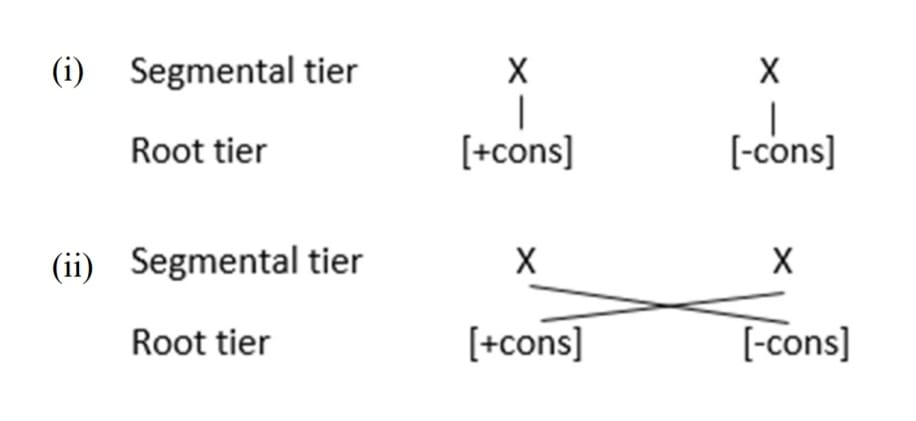
\includegraphics[width=0.5\columnwidth]{figs/Q.111.jpeg}
\label{Q.111}
\end{figure}
\begin{enumerate}
\begin{multicols}{2}
\item Representation (i)
\item Representation (ii)
\item Both (i) and (ii)
\item Neither (i) nor (ii)
\end{multicols}
\end{enumerate}
\hfill\textbf{(GATE-XH-2022)}

\item In the given sentences, the semantic relationship of hyponymy can be found in between

(i) The thing in the grass is a small snake.

(ii) The thing in the grass is a small reptile.
\begin{enumerate}
\begin{multicols}{2}
\item reptile : grass
\item grass : snake
\item snake : reptile
\item small : snake
\end{multicols}
\end{enumerate}
\hfill\textbf{(GATE-XH-2022)}

\item Which of the followings occurred due to the Great Vowel Shift of the English language?
\begin{enumerate}
\item \textipa{[a:]} became \textipa{[u:]}
\item All the front vowels shifted to back
\item \textipa{[ge:s]} became \textipa{[gi:s]}
\item The high, long vowels became diphthongized
\end{enumerate}
\hfill\textbf{(GATE-XH-2022)}

\item Which of the following statements are true for the pulmonic consonant table in an IPA chart?
\begin{enumerate}
\item Voiceless consonants aligned to the left of the cell
\item Places of articulation are arranged in rows
\item Manners of articulation are arranged in columns
\item The most constricted consonants to the least are arranged from the top to bottom
\end{enumerate}
\hfill\textbf{(GATE-XH-2022)}

\item Identify the compounds in the given data.
\begin{multicols}{5}
    repeat blackboard toyfactory underestimate deform, backward bystander, sky-high
\end{multicols}
\begin{enumerate}
\begin{multicols}{2}
\item repeat and backward
\item blackboard and toy factory
\item sky-high and underestimate
\item bystander and deform
\end{multicols}
\end{enumerate}
\hfill\textbf{(GATE-XH-2022)}

\item In the production of the /z/ sound which of the following will take place?
\begin{enumerate}
\item Vocal cords will vibrate
\item Velum will be raised
\item The two lips will be in contact
\item Air will pass without any turbulence
\end{enumerate}
\hfill\textbf{(GATE-XH-2022)}

\item The phrase “the first person in space” refers to Yuri Gagarin. Which of the following could be used to determine reference?
\begin{enumerate}
\begin{multicols}{2}
\item Russell’s Theory of Description
\item Prototype Theory
\item Speech Act Theory
\item Gricean Maxims
\end{multicols}
\end{enumerate}
\hfill\textbf{(GATE-XH-2022)}

\item Which of the following statement(s) apply to pidgins?
\begin{enumerate}
\item Pidgins have complex grammatical rules
\item Pidgins do NOT have grammatical rules
\item Pidgin phonology is rule based
\item Pidgins are passed on from one generation to the other
\end{enumerate}
\hfill\textbf{(GATE-XH-2022)}

\item In the given tree-structure NP1 C-commands NP2 but not vice versa because:
\begin{figure}[h!]
    \centering
    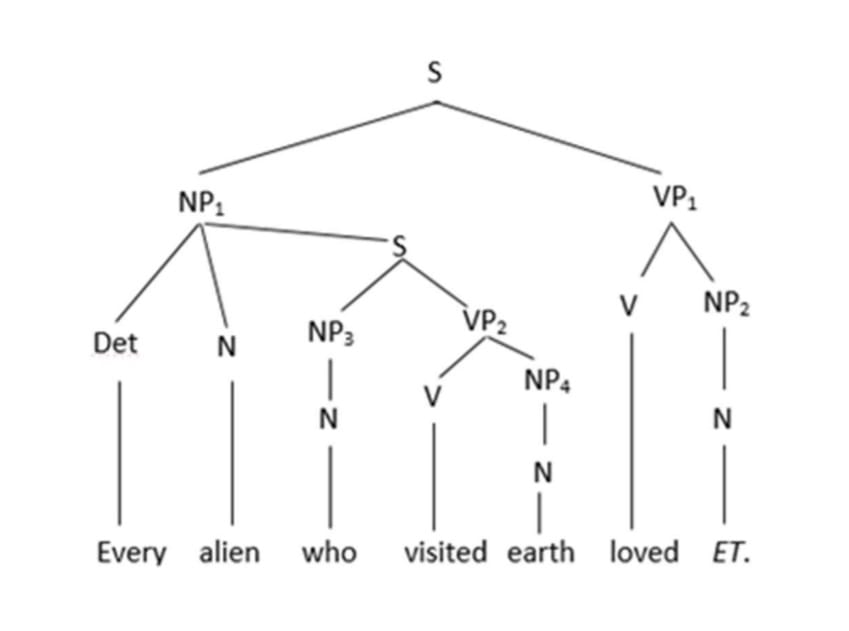
\includegraphics[width=0.5\columnwidth]{figs/Q.119.jpeg}
    \label{Q.119}
\end{figure}
\newpage
\begin{enumerate}
\item C-command cannot be a reciprocal relationship
\item No node dominates both NP2 and NP1
\item VP1 dominates NP2 and C-commands NP1
\item VP1 dominates NP2 but not NP1
\end{enumerate}
\hfill\textbf{(GATE-XH-2022)}

\item Which of the given pronunciations DO NOT conform to the phonological rule?

\sbrak{-sonorant+voice} $\;\rightarrow\;$ \sbrak{-sonorant-voice} /\underline{\hspace{0.7cm}}\#
\begin{enumerate}
\begin{multicols}{4}
\item dud
\item kut
\item mutab
\item pum
\end{multicols}
\end{enumerate}
\hfill\textbf{(GATE-XH-2022)}
\subsection*{\underline{\textbf {Q.121 – Q.141 Carry TWO marks Each}}}

\item Determine the correct nature of the following two utterances from the choices given below.  

P: Hasnain said ki woh kal aayegaa \\
(COMPL he tomorrow come.will) \\
“Hasnain said that he will come tomorrow” \\

Q: Rohan will get some desi vegetables. (local) \\
“Rohan will get some local vegetables”  
\begin{enumerate}
\item Code switching in P and Q  
\item Borrowing in P and Q  
\item Code switching in P and borrowing in Q  
\item Borrowing in P and code switching in Q  
\end{enumerate}
\hfill\textbf{(GATE-XH-2022)}

\item Consider the given script showing a sequence of 11 graphemes. It represents the sentence: /apa pal talip tani mil/. Each grapheme in the script contains a \underline{\hspace{2cm}}.
\begin{figure}[h!]
    \centering
    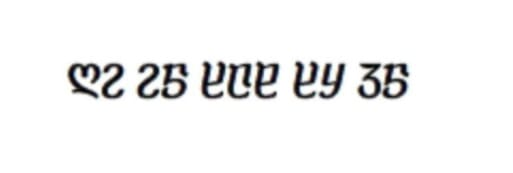
\includegraphics[width=0.5\columnwidth]{figs/Q.122.jpeg}
    \label{Q.122}
\end{figure}
\begin{multicols}{4}
\begin{enumerate}
\item Rhyme  
\item Syllable  
\item Consonant  
\item Mora  
\end{enumerate}
\end{multicols}
\hfill\textbf{(GATE-XH-2022)}

\item In the given examples, column Y are examples of \underline{\hspace{2cm}} sentences.  
\begin{tabular}{|p{5cm}|p{6cm}|}
\hline
   X  &  Y\\
   \hline
    The cat chased the rat. & It is the cat that chased the rat.\\
    \hline
    The athelete broke the record. & It is the athelete that broke the record.\\
    \hline
\end{tabular}
\begin{multicols}{4}
\begin{enumerate}
\item Topicalization  
\item Cleft  
\item Pseudo-cleft  
\item Gapping  
\end{enumerate}
\end{multicols}
\hfill\textbf{(GATE-XH-2022)}

\item A second language speaker uses the word [phonetic] as a singular noun because she interprets the word [phonetics] as a plural noun. In doing so, she is deducing a new word by the process of \underline{\hspace{2cm}}.
\begin{multicols}{4}
\begin{enumerate}
\item Blocking  
\item Back formation  
\item Bracketing  
\item Back tracking  
\end{enumerate}
\end{multicols}
\hfill\textbf{(GATE-XH-2022)}
\item Given the rules P and Q, what is the name of the rule ordering in dialect X and Y?  
\begin{figure}[h!]
    \centering
    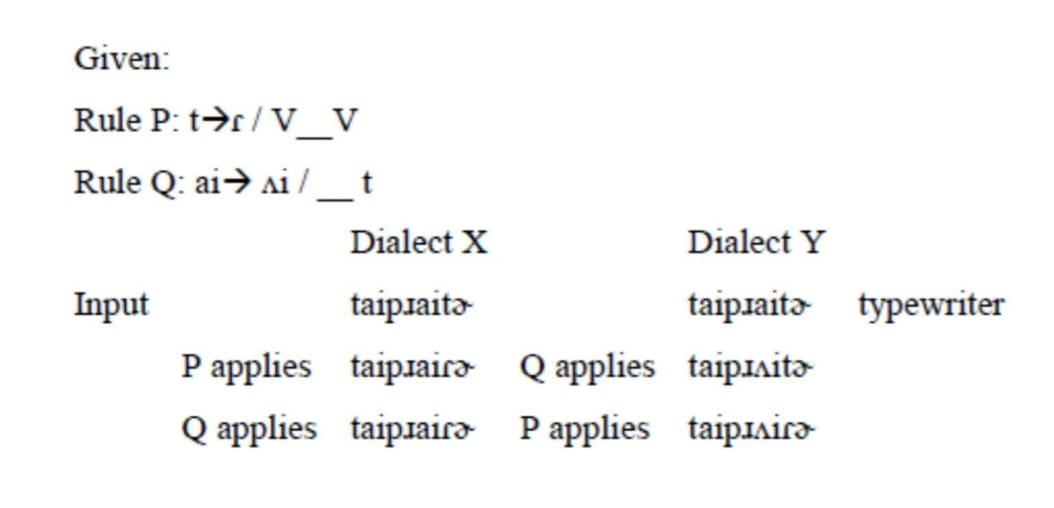
\includegraphics[width=0.6\columnwidth]{figs/Q.125.jpeg}
    \label{Q.125}
\end{figure}
\begin{enumerate}
\item X has counter-feeding and Y has counter bleeding order  
\item X has bleeding and Y has counter-bleeding order  
\item X has counter-bleeding and Y has counter-feeding order  
\item X has counter bleeding and Y has bleeding order  
\end{enumerate}
\hfill\textbf{(GATE-XH-2022)}

\item Which of the given statements is/are TRUE?  

Statement (I): Diglossia and dialect continuum are synonymous. \\
Statement (II): Bilingual speakers are also bidialectal.  

\begin{enumerate}
\item Both statement (I) and statement (II) are correct  
\item Both statement (I) and statement (II) are incorrect  
\item Statement (I) is correct but statement (II) is incorrect  
\item Statement (I) is incorrect but statement (II) is correct  
\end{enumerate}
\hfill\textbf{(GATE-XH-2022)}

\item Look into the data from Micaocan Aztec and match the words (P-S) to their meaning (i-iv) and select the correct sequence.\\
\begin{tabular}{c c c c}
nokali& my house& nokalimes &my houses\\
mokali& your house& ikali& his house\\
nokwahmili& my cornfield& mokwahmili &your cornfield\\
ikwahmili& his cornfield& nomakhwames& my friends\\
mopelomes &your dogs& mopelo& your dog\\
\end{tabular}
\begin{tabular}{|p{2cm}|p{2cm}|}
\hline
   P.kali  & (i)friend \\
   \hline
   Q.pelo  & (ii)dog\\
   \hline
   R.kwahmili &(iii)cornfield\\
   \hline
   S.makhwa & (iv)house\\
   \hline
\end{tabular}
\begin{multicols}{2}
\begin{enumerate}
\item P-(ii), Q-(iv), R-(i), S-(iii)  
\item P-(iv), Q-(ii), R-(i), S-(iii)  
\item P-(ii), Q-(iv), R-(iii), S-(i)  
\item P-(iv), Q-(ii), R-(iii), S-(i)  
\end{enumerate}
\end{multicols}
\hfill\textbf{(GATE-XH-2022)}

\item Match the languages (P–U) to the language families (i–iv) and select the correct sequence.\\ 
\begin{tabular}{|p{3cm}|p{4cm}|}
\hline
   Languages  & Language Families \\
   \hline
   P.Kannada  & (i)Indo-Aryan\\
   \hline
   Q. Assamese & (ii) Dravidian\\
   \hline
   R. Khasi & (iii) Tibeta-Burman\\
   \hline
   S. Nepali & (iv)Austo-Asiatic\\
   \hline
   T.Manipuri & \\
   \hline
   U.Mundari & \\
   \hline
\end{tabular}
\begin{multicols}{2}
\begin{enumerate}
\item P–(ii),Q–(i),R–(iv),S–(i),T-(iii),U-(iv)  
\item P–(i),Q–(i),R–(iii),S–(iii),T–(iv),U–(i)  
\item P–(ii),Q–(i),R–(iii),S–(i),T–(iii),U–(iv)  
\item P–(i),Q–(i),R–(iv),S–(iii),T–(iii),U–(ii)  
\end{enumerate}
\end{multicols}
\hfill\textbf{(GATE-XH-2022)}

\item Which of the given statements is/are TRUE?  

Statement (I): The International Phonetic Alphabet (IPA) is a transcription system for describing human speech sounds from all languages. \\
Statement (II): The voiceless pharyngeal plosive sound is missing in the IPA chart because it is physiologically impossible to articulate.  
\begin{enumerate}
\item Both statement (I) and statement (II) are correct  
\item Both statement (I) and statement (II) are incorrect  
\item Statement (I) is correct but statement (II) is incorrect  
\item Statement (I) is incorrect but statement (II) is correct  
\end{enumerate}
\hfill\textbf{(GATE-XH-2022)}

\item Match the terms in column X (P–S) to their descriptions in column Y (i–iv) and select the correct sequence.  \\
\begin{tabular}{p{3cm} p{9cm}}
    Column X  &Column Y\\
P. Competence &i. one of the different meanings of an expression\\
Q. Performance &ii. actual speech in a communicative context\\
R. Sense &iii. relation between an expression and its real world entity\\
S. Reference &iv. native speaker intuition
\end{tabular}
\begin{multicols}{2}
\begin{enumerate}
\item P – ii, Q – iv, R – iii, S – i  
\item P – iv, Q – ii, R – iii, S – i  
\item P – ii, Q – iv, R – i, S – iii  
\item P – iv, Q – ii, R – i, S – iii  
\end{enumerate}
\end{multicols}
\hfill\textbf{(GATE-XH-2022)}

\item Match the following morphological changes (P-S) to their type (i-iv) and select the correct sequence.\\
\begin{tabular}{p{4cm}|p{6cm}}
   P.electric$\rightarrow$ electricity  & (i) partial suppletion \\
   Q.go$\rightarrow$ went  & (ii) total suppletion \\
   R.ox$\rightarrow$ oxen &  (iii) lexically \\
   S.think$\rightarrow$ thought & (iv) phonologically conditioned\\
\end{tabular}
\begin{multicols}{2}
\begin{enumerate}
\item P – (ii), Q – (iv), R – (i), S – (iii)  
\item P – (iv), Q – (ii), R – (i), S – (iii)  
\item P – (ii), Q – (iv), R – (iii), S – (i)  
\item P – (iv), Q – (ii), R – (iii), S – (i)  
\end{enumerate}
\end{multicols}
\hfill\textbf{(GATE-XH-2022)}

\item Which of the given statements is/are TRUE? 
\begin{figure}[h!]
    \centering
    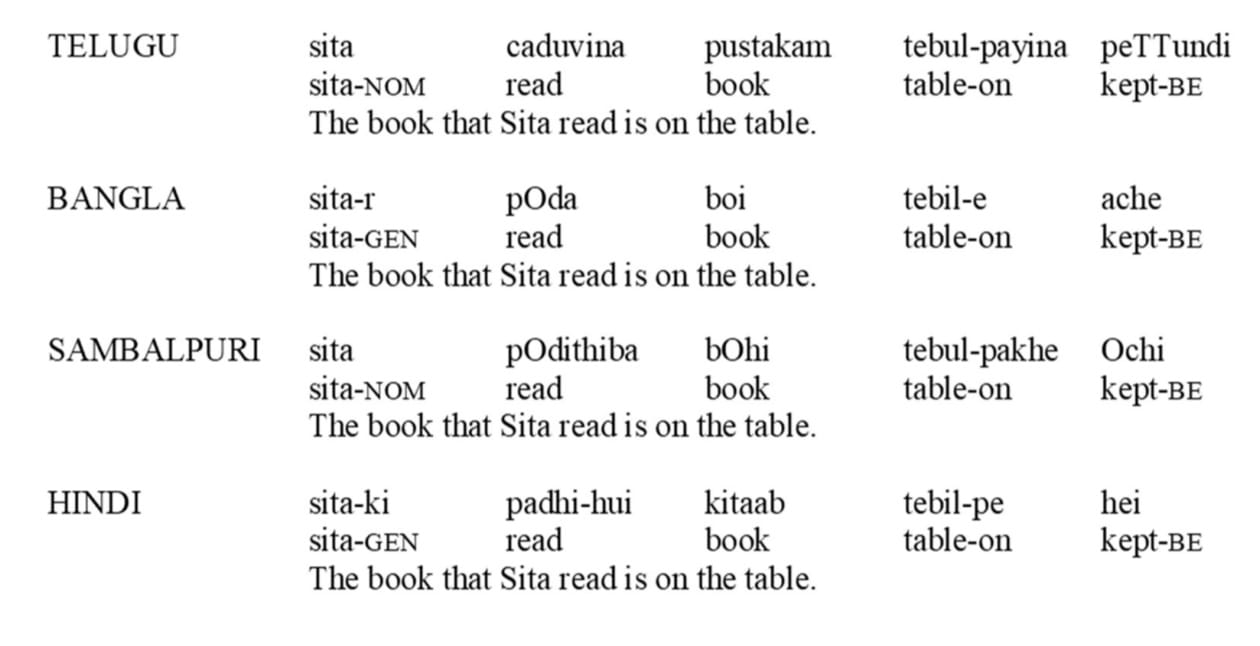
\includegraphics[width=0.9\columnwidth]{figs/Q.132.jpeg}
    \label{Q.132}
\end{figure}
\begin{enumerate}
\item Bangla is similar to Hindi and Sambalpuri but not Telugu.  
\item Bangla is similar to Hindi but not Sambalpuri.  
\item Sambalpuri is similar to Telugu but not Bangla.  
\item Sambalpuri is similar to Hindi but not Bangla.  
\end{enumerate}
\hfill\textbf{(GATE-XH-2022)}

\item Lesions in different areas of the left hemisphere lead to qualitatively distinct aphasia syndromes. Which of the given statements is/are TRUE?  
\begin{enumerate}
\item The brain lesions associated with classical anomia involves the dominant angular gyrus.  
\item Conduction aphasia follows from a lesion in the posterior part of the inferior frontal gyrus.  
\item Wernicke’s aphasia is the consequence of a lesion in the auditory association cortex of the temporal lobe.  
\item Broca’s aphasia follows from localized lesions in the temporoparietal regions.  
\end{enumerate}
\hfill\textbf{(GATE-XH-2022)}

\item Consider the following data from English. Which linguistic change(s) is/are associated with the addition of the suffix ‘-able’?  

This book is readable.  
\begin{multicols}{2}
\begin{enumerate}
\item Sociolinguistic change  
\item Grammatical category change  
\item Semantic change  
\item Typological change  
\end{enumerate}
\end{multicols}
\hfill\textbf{(GATE-XH-2022)}

\item Children are biologically equipped to acquire all aspects of grammar. Which of the given statements is/are TRUE? 
\begin{enumerate}
\item ‘Telegraphic speech’ occurs during the holophrastic stage.  
\item Children generally go through three phases in the acquisition of an irregular form (overgeneralization).  
\item Children learn approximately 100 words a day up to 12 months.  
\item Mean length of utterances is used to measure a child’s language development.  
\end{enumerate}
\hfill\textbf{(GATE-XH-2022)}

\item Wolof speakers use a secret language called Kall. Words in Wolof are changed to Kall in a systematic manner, as shown in the data. In the change from Wolof to Kall, which of the given constraints cannot be violated?\\
    Wolof \hspace{1cm}  Kall \hspace{1cm}  Gloss\\
    sama \hspace{1cm}  masa \hspace{1cm}   my\\
    jabar\hspace{1.2cm} barja \hspace{1cm}  wife\\
    ker \hspace{1.3cm}  reke  \hspace{1cm} home
    
\begin{multicols}{2}
\begin{enumerate}
\item MAX-IO  
\item DEP-IO  
\item FOOT-BINARITY  
\item LINEARITY-IO  
\end{enumerate}
\end{multicols}
\hfill\textbf{(GATE-XH-2022)}

\item The given sentence is ungrammatical because:  

*Tailan believes that himself is smarter than Po  
\begin{enumerate}
\item Principle A of Binding Theory is not satisfied.  
\item Principle B of Binding Theory is not satisfied.  
\item Principle C of Binding Theory is not satisfied.  
\item Both Po and Tailan are possible antecedents for himself. 
\end{enumerate}
\hfill\textbf{(GATE-XH-2022)}


\item Which of the given statements support the Design Features proposed by Hockett?  
\begin{enumerate}
\item Humans produce as many sentences as they have acquired.  
\item Sentences cannot be broken into smaller units as they have specific meaning.  
\item Humans can talk about things that are not in their immediate vicinity.  
\item Linguistic units do not bear any direct resemblance to the things they represent.  
\end{enumerate}
\hfill\textbf{(GATE-XH-2022)}

\item Which of the given logical forms correspond to the following sentence where x $\in$ student, y $\in$ teacher and A=admires?  

Every student admires a teacher.  
\begin{multicols}{4}
\begin{enumerate}
\item $\forall x \exists y \; A(x,y)$  
\item $\forall y \exists x \; A(y,x)$  
\item $\exists x \forall y \; A(y,x)$  
\item $\exists y \forall x \; A(x,y)$  
\end{enumerate}
\end{multicols}
\hfill\textbf{(GATE-XH-2022)}

\item Identify the possible set(s) of stops that correlate with the corresponding VOT values.  
\begin{multicols}{2}
\begin{enumerate}
\item /p/ = 10, /ph/ = 78, /b/ = –110  
\item /t/ = 120, /th/ = –110, /d/ = 67  
\item /k/ = –121, /kh/ = 121, /g/ = –108  
\item /ph/ = 89, /th/ = 92, /kh/ = 98  
\end{enumerate}
\end{multicols}
\hfill\textbf{(GATE-XH-2022)}


\item The estimated fundamental frequency of the given sine wave is (in integer) \underline{\hspace{2cm}} Hz.  

\begin{figure}[h!]
\centering
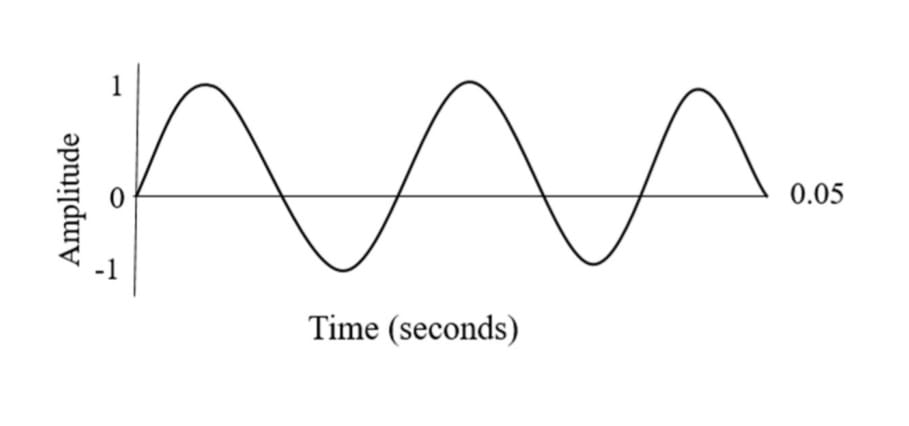
\includegraphics[width=0.5\columnwidth]{figs/Q.141.jpeg}
\label{Q.141}
\end{figure}
\hfill\textbf{(GATE-XH-2022)}
\newpage
\section*{\large \underline{\textbf {GATE 2022 PHILOSOPHY (XH C4)}}}
\subsection*{\underline{\textbf {XH-C4 (Q.142 – Q.159 Carry ONE mark Each)}}}

\item Let us consider the cases of Shweta and Rani. While Shweta has access to, and can afford to buy good quality dairy products, she and her spouse decide to pursue a vegan lifestyle. Therefore, she no longer buys milk or dairy-based products for her family. Rani’s family on the other hand, has a meagre income. Although Rani’s children like milk and kheer, Rani refrains from buying milk and instead spends on rice.\\  
In light of the concepts of functioning and capability as defined by Martha Nussbaum, which one of the following options holds for the above cases?  
\begin{enumerate}
\item They differ on the basis of capability  
\item They differ on the basis of functioning  
\item They differ on the basis of both functioning and capability  
\item They do not differ since the end-result is the same in both  
\end{enumerate}
\hfill\textbf{(GATE-XH-2022)}

\item In the opposition of propositions, which one among the following is the contradictory of A proposition?  
\begin{multicols}{4}
\begin{enumerate}
\item Only O  
\item Only E  
\item Only I  
\item E and O  
\end{enumerate}
\end{multicols}
\hfill\textbf{(GATE-XH-2022)}

\item A study in Europe concluded that whenever there is an increase in the circulation of fake news in social media, the ruling party gains political mileage. Conversely, a proportionate decrease in the circulation of fake news, corresponds to the decline in its popularity.\\  
Which one of Mill’s methods is entailed in the above reasoning?  
\begin{enumerate}
\item Method of Concomitant Variation  
\item Joint Method of Agreement and Difference  
\item Method of Residues  
\item Method of Difference  
\end{enumerate}
\hfill\textbf{(GATE-XH-2022)}

\item Which one among the following Greek philosophers upholds the ontology of things by stating that ‘all things are flowing’ and ‘nothing ever is, everything is becoming?’  
\begin{multicols}{4}
\begin{enumerate}
\item Heraclitus  
\item Pythagoras  
\item Thales  
\item Anaxagoras  
\end{enumerate}
\end{multicols}
\hfill\textbf{(GATE-XH-2022)}

\item Which one among the following will be in agreement with Rene Descartes’ confirmation of the cogito, in his \textit{Discourse on Method}?  
\begin{multicols}{2}
\begin{enumerate}
\item Self exists as an imperfect thing  
\item Self exists as a perfect thing  
\item Only the world exists  
\item Only the self exists  
\end{enumerate}
\end{multicols}
\hfill\textbf{(GATE-XH-2022)}

\item According to Immanuel Kant, duty as rationally conceived is determined by:
\begin{enumerate}
\item The will as an a priori principle  
\item The self-interest of the will  
\item The divine will  
\item The desire as the will
\end{enumerate}
\hfill\textbf{(GATE-XH-2022)}

\item Which one among the following is NOT a pramāṇa in Sānkhya epistemology?  
\begin{multicols}{2}
\begin{enumerate}
\item Comparison (upamāna)  
\item Perception (dṛṣta/pratyakṣa)  
\item Inference (anumāna)  
\item Valid testimony (āptavacana)  
\end{enumerate}
\end{multicols}
\hfill\textbf{(GATE-XH-2022)}

\item ‘Hare’s horn (śaśa-viṣāṇa)’, according to the Philosophy of Yoga, is a valid example of which kind of citta-vṛtti?  
\begin{enumerate}
\item Constructive Imagination (vikalpa)  
\item Wrong cognition or false knowledge (viparyaya)  
\item Absence of cognition or sleep (nidra)  
\item Memory (smṛti)  
\end{enumerate}
\hfill\textbf{(GATE-XH-2022)}

\item According to Jaimini, in Mīmāṃsā, which one among the following is a command or injunction that impels humans to perform action?  
\begin{multicols}{4}
\begin{enumerate}
\item Dharma  
\item Apūrva  
\item Adṛṣṭa  
\item Niṣkāmakarma  
\end{enumerate}
\end{multicols}
\hfill\textbf{(GATE-XH-2022)}

\item According to Vaiśeṣika theory of atomism, which one of the following is NOT atomic?  
\begin{multicols}{4}
\begin{enumerate}
\item Ether (ākāśa)  
\item Earth (pṛthvi)  
\item Fire (tejas)  
\item Air (vāyu)  
\end{enumerate}
\end{multicols}
\hfill\textbf{(GATE-XH-2022)}

\item The Cārvāka system rejects inference (anumāna) as a pramāṇa because it does not accept:  
\begin{multicols}{2}
\begin{enumerate}
\item Invariable concomitance (vyāpti)  
\item Comparison (upamāna) as a pramāṇa  
\item The theory of pramāṇa altogether  
\item Śabda as a pramāṇa  
\end{enumerate}
\end{multicols}
\hfill\textbf{(GATE-XH-2022)}

\item The Muṇḍakopaniṣad distinguishes between ‘higher knowledge’ (parā vidyā) and ‘lower knowledge’ (aparā vidyā). What does the higher knowledge (parā vidyā) imply?  
\begin{multicols}{2}
\begin{enumerate}
\item Knowledge of the Ātman  
\item Knowledge of the World  
\item Knowledge of Karma  
\item Knowledge of God  
\end{enumerate}
\end{multicols}
\hfill\textbf{(GATE-XH-2022)}

\item In the Bhagavadgītā, the conception of ‘lokasamgraha’ denotes that the perfect person:  
\begin{enumerate}
\item Purely acts for the wellbeing and welfare of humanity  
\item Purely concentrates on the Absolute by negating the world  
\item Fully detaches herself/himself from worldly affairs  
\item Fully devotes herself/himself to speak about God to people  
\end{enumerate}
\hfill\textbf{(GATE-XH-2022)}

\item S. Radhakrishnan, in his \textit{An Idealistic View of Life}, delineates the nature of ultimate reality as “pure consciousness, pure freedom and infinite possibility.” Which school of Indian Philosophy influenced him most?  
\begin{enumerate}
\begin{multicols}{4}
\item Advaita Vedānta  
\item Sānkhya  
\item Cārvāka  
\item Mīmāṃsā 
\end{multicols}
\end{enumerate}
\hfill\textbf{(GATE-XH-2022)}

\item Karl Marx in his \textit{Economic and Philosophic Manuscripts} discusses various forms of alienation within capitalist society. Which of the following appear(s) in Marx’s list of alienation?  
\begin{multicols}{2}
\begin{enumerate}
\item From the product of one’s labour  
\item From one’s species-being  
\item From one another  
\item From one’s natural rights  
\end{enumerate}
\end{multicols}
\hfill\textbf{(GATE-XH-2022)}

\item Which among the following option(s) define(s) the nature of Forms according to Plato?  
\begin{multicols}{2}
\begin{enumerate}
\item Non-mental  
\item Independent of particulars  
\item Temporal  
\item Residing in God  
\end{enumerate}
\end{multicols}
\hfill\textbf{(GATE-XH-2022)}

\item Jīva and Ajīva are the Categories (padārtha) in Jainism. Which of the following are included in Ajīva?  
\begin{multicols}{2}
\begin{enumerate}
\item Matter (pudgala)  
\item Space (ākāśa)  
\item Motion (dharma)  
\item Cause (hetu)  
\end{enumerate}
\end{multicols}
\hfill\textbf{(GATE-XH-2022)}

\item In the Śaivasiddhānta, the Supreme Reality is called Pati, the individual self/soul is called Paśu, and the fetters which bind the souls are called Pāśa. Which of the following are included in Pāśa?  
\begin{multicols}{4}
\begin{enumerate}
\item Karma  
\item Māyā  
\item Kāma  
\item Moha  
\end{enumerate}
\end{multicols}
\hfill\textbf{(GATE-XH-2022)}
\subsection*{\underline{\textbf{Q.160 – Q.180 Carry TWO marks Each}}}

\item Read the passage carefully and answer the question:\\
“Only, unlike Kant, we do not see man as being essentially a positive will. On the contrary, he is first defined as a negativity. He is first at a distance from himself. He can coincide with himself only by agreeing never to rejoin himself. There is within him a perpetual playing with the negative, and he thereby escapes himself, he escapes his freedom. And it is precisely because an evil will is here possible that the words “to will oneself free” have a meaning. Therefore, not only do we assert that the existentialist doctrine permits the elaboration of an ethics, but it even appears to us as the only philosophy in which an ethics has its place. For, in a metaphysics of transcendence, in the classical sense of the term, evil is reduced to error; and in humanistic philosophies it is impossible to account for it, man being defined as complete in a complete world. Existentialism alone gives – like religions – a real role to evil, and it is this, perhaps, which make its judgments so gloomy. Men do not like to feel themselves in danger.”

\hfill --- Simone de Beauvoir, \textit{The Ethics of Ambiguity}

Which one of the following claim is made in the passage regarding Existentialism?
\begin{enumerate}
\item Its emphasis on negativity means that it can account for evil.  
\item It cannot give rise to an ethic since it rejects the idea of evil.  
\item It believes that evil is a kind of error.  
\item It must withhold judgments about evil.  
\end{enumerate}
\hfill\textbf{(GATE-XH-2022)}

\item Keeping in mind the central commitments of John Dewey’s Pragmatism, which one of the following applies to his concept of experience?
\begin{enumerate}
\item It involves transaction between the individual and her environment.  
\item It is an inferior source of knowledge.  
\item It is shaped by the environment but cannot modify the environment.  
\item It is overridden by reason in validating knowledge.  
\end{enumerate}
\hfill\textbf{(GATE-XH-2022)}

\item All Covid-19 patients are fighters. No Covid-19 patients are children. Therefore, no children are fighters.  

Which one among the following options determines the mood, figure, and fallacy of the above argument?  
\begin{multicols}{2}
\begin{enumerate}
\item AEE, III Figure, Illicit Major  
\item AEE, II Figure, Undistributed Middle  
\item AEE, III Figure, Illicit Minor  
\item AEE, II Figure, Existential Fallacy  
\end{enumerate}
\end{multicols}
\hfill\textbf{(GATE-XH-2022)}

\item In the theory of causation, the effect (\textit{kārya}) is non-existent (asat) before its creation; it is a new beginning (\textit{ārambha}). Which one of the following schools of thought in Indian philosophy upholds this theory?
\begin{multicols}{4}
\begin{enumerate}
\item Nyāya  
\item Vedānta  
\item Yoga  
\item Sānkhya  
\end{enumerate}
\end{multicols}
\hfill\textbf{(GATE-XH-2022)}

\item Read the passage carefully and answer the question:\\
“Passive resistance is a method of securing rights by personal suffering; it is the reverse of resistance by arms. When I refuse to do a thing that is repugnant to my conscience, I use soul-force. For instance, the Government of the day has passed a law which is applicable to me. I do not like it. If by using violence I force the Government to repeal the law, I am employing what may be termed body-force. If I do not obey the law and accept the penalty for its breach, I use soul-force. It involves sacrifice of self.”\\
\hfill --- M. K. Gandhi, \textit{Hind Swaraj or Indian Home Rule}

Which one among the following is NOT in conformity with the above passage?
\begin{multicols}{2}
\begin{enumerate}
\item Soul-force is brute force  
\item Passive resistance involves sacrifice  
\item Conscience is the soul-force  
\item Active resistance is body-force  
\end{enumerate}
\end{multicols}
\hfill\textbf{(GATE-XH-2022)}

\item In light of Merleau-Ponty’s concepts of the body and perception, which of the following claim(s) is/are true about my body?
\begin{enumerate}
\item It is the vantage-point of my perception.  
\item It is the subject of perception.  
\item It can appear in my perception just like other objects.  
\item It is not embedded in my field of perception.  
\end{enumerate}
\hfill\textbf{(GATE-XH-2022)}

\item Plato's theory of recollection sheds light on the origins of knowledge. Which among the following option(s) does it intend to explain?
\begin{enumerate}
\item Philosophical and mathematical discoveries  
\item Our linguistic capacities  
\item Innateness of knowledge  
\item Only higher learning but not the ordinary learning  
\end{enumerate}
\hfill\textbf{(GATE-XH-2022)}

\item Which among the following is/are correct statement(s) about Aristotle’s approach to the study of logic and its contribution to science (\textit{episteme})?
\begin{enumerate}
\item Logic is a mere tool and not an end in itself.  
\item Logic makes an important but incomplete contribution to science.  
\item The mind-independent nature of things is not accessible only through Logic.  
\item Science employs only Deductive Logic.  
\end{enumerate}
\hfill\textbf{(GATE-XH-2022)}

\item Which among the following statement(s) is/are in accordance with John Locke’s epistemological concern in his \textit{Essay Concerning Human Understanding}?

\begin{enumerate}
\item All our knowledge ultimately derives from experience.  
\item Experience immediately provides us with ideas, not knowledge as such.  
\item Reason has no role to play in our acquisition of knowledge.  
\item Our knowledge has no limits.  
\end{enumerate}
\hfill\textbf{(GATE-XH-2022)}

\item Which among the following fundamental rationalist beliefs concerning the cause and effect relation does David Hume reject?
\begin{enumerate}
\item Causes contain their effects.  
\item Causes entail their effects.  
\item There is necessary connection between cause and effect.  
\item Causal reasoning is not like demonstrative reasoning.  
\end{enumerate}
\hfill\textbf{(GATE-XH-2022)}

\item If Immanuel Kant is said to have brought about a Copernican revolution in philosophy, it is because:
\begin{enumerate}
\item For bringing foundational change in metaphysics.  
\item For showing that objects conform to perception and not perception to objects.  
\item For placing mind at the center of epistemology.  
\item For bringing foundational change in the theory of morality.  
\end{enumerate}
\hfill\textbf{(GATE-XH-2022)}

\item What differentiates Logical Positivism of the Vienna Circle from earlier forms of Empiricism and Positivism of Hume, Mach, Comte and Mill?
\begin{enumerate}
\item In holding that the ultimate basis of knowledge rests upon public experimental verification rather than personal experience.  
\item In holding that metaphysical doctrines are not false but meaningless.  
\item In holding that all genuine knowledge about nature can be expressed in a single language common to all the sciences.  
\item In confirming the possibility of synthetic a priori.  
\end{enumerate}
\hfill\textbf{(GATE-XH-2022)}

\item Bertrand Russell’s philosophy of Logical Atomism intends to establish his methodological and metaphysical standpoints. Which among the following is/are in accordance with his doctrine?
\begin{enumerate}
\item Everything we experience can be analyzed into logical atoms.  
\item Logical atoms are particulars, qualities, and relations.  
\item Logical atoms are universals, and not about qualities and relations.  
\item We can apprehend reality as it is in itself, unaffected by the medium of thought.  
\end{enumerate}
\hfill\textbf{(GATE-XH-2022)}

\item Using the theories of punishment to argue for or against capital punishment, which among the following is/are true?
\begin{enumerate}
\item A combination of Utilitarian and Deterrent theories will argue for capital punishment.  
\item A combination of Utilitarian and Retributive theories will argue for capital punishment.  
\item A combination of Utilitarian and Reformative theories will argue against capital punishment.  
\item A combination of Reformative and Retributive theories will argue against capital punishment.  
\end{enumerate}
\hfill\textbf{(GATE-XH-2022)}

\item Gilbert Ryle believed that Descartes’ mind-body dualism commits a category mistake. Which of the following motive(s) of Descartes lead(s) to this category mistake?
\begin{enumerate}
\item Endorsement of the claims of mechanics but not the Hobbesian kind  
\item Belief in religion and morality  
\item The mental cannot be a variety of the mechanical  
\item Complete endorsement of Hobbesian mechanics  
\end{enumerate}
\hfill\textbf{(GATE-XH-2022)}

\item Ludwig Wittgenstein, in his \textit{Tractatus Logico-Philosophicus}, writes, “A picture can depict any reality whose form it has.” Which of the following proposition(s) will be in line with this?
\begin{enumerate}
\item A picture can always display a pictorial form.  
\item A picture has logical form.  
\item A logical picture can depict the world.  
\item A picture can depict its pictorial form.  
\end{enumerate}
\hfill\textbf{(GATE-XH-2022)}

\item Select the CORRECT combinations of the Vedanta schools and their propounders:
\begin{multicols}{2}
\begin{enumerate}
\item Dvaita --- Madhva  
\item Śuddhādvaita --- Rāmānuja  
\item Advaita --- Śaṅkara  
\item Viśiṣṭādvaita --- Nimbārka  
\end{enumerate}
\end{multicols}
\hfill\textbf{(GATE-XH-2022)}

\item Which of the following is/are part of the six \textit{pāramitās} (ṣaḍpāramitā) in Buddhism?
\begin{multicols}{2}
\begin{enumerate}
\item Charity or giving (\textit{dāna})  
\item Virtuous conduct (\textit{śīla})  
\item Forbearance or patience (\textit{kṣānti})  
\item Non-violence (\textit{ahimsā})  
\end{enumerate}
\end{multicols}
\hfill\textbf{(GATE-XH-2022)}

\item Read the passage carefully and answer the question:

“Habits of the constitutional morality may be essential for the maintenance of a constitutional form of government. But the maintenance of a constitutional form of Government is not the same thing as a self-government by the people. Similarly, it may be granted that adult suffrage can produce government of the people in the logical sense of the phrase, i.e., in contrast to the government of a king. But it cannot by itself be said to bring about a democratic government, in the sense of the government by the people and for the people.”\\
\hfill --- B.R. Ambedkar, "Democracy" \textit{The Essential Writings of B. R. Ambedkar}\\
Which of the following statements is/are NOT in conformity with the passage?
\begin{enumerate}
\item The maintenance of self-governance is always maintenance of constitutional government.  
\item Constitutional morality may not be essential for preservation of constitutional form of government.  
\item Adult suffrage itself is sufficient to bring about a democratic government.  
\item Elected government is logically in contrast to the government of a king.  
\end{enumerate}
\hfill\textbf{(GATE-XH-2022)}

\item Read the passage carefully and answer the question:\\
“What do I mean by the ideal of universal religion? I do not mean any one universal philosophy, or any one universal mythology, or any one universal ritual held by all; for I know that this world must go on working, wheel within wheel, this intricate mass of machinery, most complex, most wonderful. What can we do then? We can make it run smoothly, we can lessen the friction; we can grease the wheels, as it were. How? By recognizing natural necessity of variation. Just as we have recognized unity by our very nature, so we must also recognize variation. We must learn that truth may be expressed in a hundred thousand ways, and that each of these ways is true as far as it goes.”\\
\hfill --- Swami Vivekananda, \textit{The Ideal of a Universal Religion}\\
Which of the following is/are characteristics of Vivekananda’s ideal of universal religion?
\begin{enumerate}
\item No adherence to any particular religion  
\item Celebration of differences  
\item Recognition of multiple truths  
\item Reduction of all religions into a single religion  
\end{enumerate}
\hfill\textbf{(GATE-XH-2022)}

\item Read the song carefully and answer the question: \\ 
Deliverance is not for me in renunciation. I feel the embrace of
freedom in a thousand bonds of delight.
Thou ever pourest for me the fresh draught of thy wine of various
colours and fragrance, filling this earthern vessel to the brim.
My world will light its hundred different lamps with thy flame and
place them before the altar of thy temple.
No, I will never shut the doors of my senses. The delights of sight
and hearing and touch will bear thy delight.
Yes, all my illusions will burn into illumination of joy, and all my
desires ripen into fruits of love.\\
\textit{(Song from Tagore’s Gitanjali is given here in original exam — omit due to copyright).}\\
The above song voices Tagore’s philosophy of life. Which among the following is/are in conformity with the message?
\begin{enumerate}
\item Denial of asceticism.  
\item Worldliness and divinity are not at odds with each other.  
\item Appreciation and enjoyment of the world.  
\item Denial of sensuous indulgence in the world.  
\end{enumerate}
\hfill\textbf{(GATE-XH-2022)}
\newpage
\section*{\large \underline{\textbf {GATE 2022 Psychology (XH-C5)}}}
\subsection*{\underline{\textbf {XH -C5 (Q.181 – Q.198 Carry ONE mark Each)}}}

\item The construct validity of a test is assessed through
\begin{enumerate}
\item Convergent and Discriminant validity
\item Concurrent and Predictive validity
\item Convergent and Predictive validity
\item Discriminant and Predictive validity
\end{enumerate}
\hfill\textbf{(GATE-XH-2022)}

\item Memory involves three stages. Find out the correct sequence from the following:
\begin{multicols}{2}
\begin{enumerate}
\item Storage, Encoding, Retrieval
\item Retrieval, Encoding, Storage
\item Encoding, Storage, Retrieval
\item Decoding, Encoding, Storage
\end{enumerate}
\end{multicols}
\hfill\textbf{(GATE-XH-2022)}

\item Erickson’s fifth stage of psychosocial development is
\begin{multicols}{2}
\begin{enumerate}
\item Identity vs role confusion
\item Intimacy vs isolation 
\item Generative vs stagnation
\item Integrity vs despair
\end{enumerate}
\end{multicols}
\hfill\textbf{(GATE-XH-2022)}

\item Test developers use reverse coding of certain items in a scale to offset the effects of
\begin{multicols}{2}
\begin{enumerate}
\item Social desirability
\item Acquiescence
\item Faking
\item Random responding
\end{enumerate}
\end{multicols}
\hfill\textbf{(GATE-XH-2022)}

\item According to Kohlberg’s theory of Moral development, at which level individuals judge morality in terms of abstract principles?
\begin{multicols}{2}
\begin{enumerate}
\item Pre-conventional
\item Post-conventional
\item Conventional
\item Transcendental
\end{enumerate}
\end{multicols}
\hfill\textbf{(GATE-XH-2022)}

\item You had been driving a car with manual-gear for 5 years. Recently, you started driving a new car with an auto-gear. If you are having any trouble, it is most likely due to
\begin{multicols}{2}
\begin{enumerate}
\item Proactive interference
\item Retroactive interference
\item Anterograde interference
\item Learning Difficulties
\end{enumerate}
\end{multicols}
\hfill\textbf{(GATE-XH-2022)}

\item Which of the following is not a behaviour therapy technique?
\begin{multicols}{2}
\begin{enumerate}
\item Flooding
\item Countertransference
\item Counterconditioning
\item Systematic desensitization
\end{enumerate}
\end{multicols}
\hfill\textbf{(GATE-XH-2022)}

\item According to Robert Sternberg, ``Street Smarts’’ refers to –
\begin{multicols}{2}
\begin{enumerate}
\item Analytical intelligence
\item Creative intelligence
\item Emotional intelligence
\item Practical intelligence
\end{enumerate}
\end{multicols}
\hfill\textbf{(GATE-XH-2022)}

\item Research design in which several age groups of participants are studied at one particular point of time is called:
\begin{multicols}{2}
\begin{enumerate}
\item Cross-sequential design
\item Functional design
\item Cross-sectional design
\item Longitudinal design
\end{enumerate}
\end{multicols}
\hfill\textbf{(GATE-XH-2022)}

\item Proximo-distal direction of development explains the nature of the development from
\begin{multicols}{2}
\begin{enumerate}
\item Top to bottom
\item Internal organs to external organs
\item Centre to periphery
\item Sensory organ to motor organs
\end{enumerate}
\end{multicols}
\hfill\textbf{(GATE-XH-2022)}

\item A cricket player who could not play an easy ball and gets out without scoring any run and blames the pitch, is an expression of 
\begin{multicols}{4}
\begin{enumerate}
\item Sublimation
\item Regression
\item Projection
\item Rationalization
\end{enumerate}
\end{multicols}
\hfill\textbf{(GATE-XH-2022)}

\item The process through which we seek to identify the causes of other’s behaviour and gain knowledge of their stable traits and dispositions is known as
\begin{multicols}{4}
\begin{enumerate}
\item Distribution
\item Dissemination
\item Retribution
\item Attribution
\end{enumerate}
\end{multicols}
\hfill\textbf{(GATE-XH-2022)}

\item Which of the following techniques is used to measure the variations in the activity of Ascending Reticular Activating System (ARAS)?
\begin{multicols}{4}
\begin{enumerate}
\item ECG
\item PET
\item fMRI
\item EEG
\end{enumerate}
\end{multicols}
\hfill\textbf{(GATE-XH-2022)}

\item The statement ``I can do no wrong, but, you can do no right’’, refers to
\begin{multicols}{2}
\begin{enumerate}
\item The self-serving bias
\item The self-other bias
\item The other-self bias
\item The other-serving bias
\end{enumerate}
\end{multicols}
\hfill\textbf{(GATE-XH-2022)}

\item Which of the following is a qualitative research design where learned experiences of individuals are examined in their life world?
\begin{multicols}{2}
\begin{enumerate}
\item Phenomenology
\item Ethnography
\item Focused-group discussion
\item Grounded-theory
\end{enumerate}
\end{multicols}
\hfill\textbf{(GATE-XH-2022)}

\item Which part of the brain is responsible for transferring information from STM to LTM?
\begin{multicols}{4}
\begin{enumerate}
\item Amygdala
\item Hypothalamus
\item Hippocampus
\item Cerebellum
\end{enumerate}
\end{multicols}
\hfill\textbf{(GATE-XH-2022)}

\item The mean of a distribution is 14 and standard deviation is 5. What would be the value of coefficient of variation? (round off to two decimal places)
\hfill\textbf{(GATE-XH-2022)}

\item Swami gets a test score of 190, the mean is 150 and SD is 25. Assuming normal distribution, the Z score would be \underline{\hspace{2cm}}. (round off to one decimal place)
\hfill\textbf{(GATE-XH-2022)}

\subsection*{\underline{\textbf {Q.199 – Q.219 Carry TWO marks Each}}}
\item
Which of the following statement(s) is/are correct regarding Multiple Analysis of Variance (MANOVA)? 
\begin{enumerate}
\item Tests the mean difference of more than two groups on one dependent variable.   
\item Tests the mean difference of more than two groups across several dependent variables.  
\item The independent variable is measured on a nominal scale and dependent variable on an interval or ratio scale. 
\item The dependent variable is measured on nominal scale and independent variable on an interval or ratio scale. 
\end{enumerate}
\hfill\textbf{(GATE-XH-2022)}

\item
Which of the following statements is/are related to observational learning? 
\begin{enumerate}
\item Remembering the steps to perform a task 
\item A person in a dinner wants to know how to use the utensils by watching others   
\item A person uses chocolate to motivate his son to perform the task 
\item A person is capable of reproducing the action after viewing it
\end{enumerate}
\hfill\textbf{(GATE-XH-2022)}

\item
Find out the statements which are related to different types of reliability?  
\begin{enumerate}
\item The same test is administered to the same people at two points in time 
\item Give the test once and have it scored by two scorers or by two methods 
\item Give the test in one administration and then split the test into two halves for scoring 
\item The extent to which people score on a measure are correlated with other variables  
\end{enumerate}
\hfill\textbf{(GATE-XH-2022)}

\item
Which of the following statement(s) regarding test scores and their interpretations is/are correct? 
\begin{enumerate}
\item Frequency distribution are graphs to help us understand the distribution of test scores 
\item Normal probability distribution is a theoretical distribution to help us understand the distribution of test scores 
\item Central tendency measures are numerical tools to help us locate the middle of a distribution of a test score 
\item Measurement of variability are numerical tools to help us understand the spread of a distribution of a test score 
\end{enumerate}
\hfill\textbf{(GATE-XH-2022)}

\item
Which of the following statement(s) is/are correct regarding the negative symptoms of schizophrenia? 
\begin{enumerate}
\item Auditory hallucination, persecution, and disorganized thinking 
\item Lack of effect in situation, poor motivation, and social withdrawal  
\item Loss of interest in day-to-day activities, lack of will, and difficulty in expressing emotions 
\item Visual hallucination, delusions of grandeur, and delusion of control
\end{enumerate}
\hfill\textbf{(GATE-XH-2022)}

\item
Which of the following statement(s) is/are correct about children with ADHD (Attention Deficit Hyperactivity Disorder)?
\begin{enumerate}
\item They have deficit in brain related executive function 
\item They have difficulty to control voluntary movements, verbal expression and problem solving due to frontal lobes  
\item Cerebellum (an area of the brain) does not work properly, which coordinates muscular activity 
\item It is also known as hypokinetic disorder 
\end{enumerate}
\hfill\textbf{(GATE-XH-2022)}

\item
Which of the following assumptions are correct about equity theory?  
\begin{enumerate}
\item Focusses on procedural justice 
\item Motivation is influenced by relative and absolute rewards 
\item Referent is the other-inside 
\item Achieving balance between input-output 
\end{enumerate}
\hfill\textbf{(GATE-XH-2022)}

\item
Which of the following statement(s) are related to Bem’s theory of self-perception? 
\begin{enumerate}
\item It starts with development of one’s basic self-concept 
\item Behaviour is a source of knowledge 
\item It is related to attitude formation 
\item It suggests that people change their attitude because of their behaviour
\end{enumerate}
\hfill\textbf{(GATE-XH-2022)}

\item
Which of the following statements are related to social cognition? 
\begin{enumerate}
\item How individuals interpret, analyze, remember and use information about the social world 
\item How people create mental structure to organise knowledge about the social world 
\item How people think about themselves and the social world  
\item It does not allow interaction between people and the environment 
\end{enumerate}
\hfill\textbf{(GATE-XH-2022)}

\item
Which of the following theory(ies) is/are related to work motivation? 
\begin{multicols}{2}
\begin{enumerate}
\item Motivation-Hygiene Theory 
\item Expectancy Theory 
\item Trait Theory 
\item ERG Theory 
\end{enumerate}
\end{multicols}
\hfill\textbf{(GATE-XH-2022)}

\item
Which of the following are not part of Thurstone’s theory of primary mental abilities? 
\begin{multicols}{2}
\begin{enumerate}
\item Numerical Ability 
\item Word Fluency 
\item Analytical Ability 
\item Short-Term Memory 
\end{enumerate}
\end{multicols}
\hfill\textbf{(GATE-XH-2022)}

\item
Which of the following are the competencies of a Bystander? 
\begin{enumerate}
\item Deciding how to help a person in need 
\item Deciding how to avoid a person at the time of his/her distress 
\item Deciding to standby with a person at the time of his/her emergency  
\item Too busy to help 
\end{enumerate}
\hfill\textbf{(GATE-XH-2022)}

\item
Which of the following functions are related to pancreas? \\
\begin{enumerate}
\item Release of hormones  
\item Converts food we eat into fuel for the body cells 
\item It regulates the level of glucose in the blood 
\item It damages digestive system 
\end{enumerate}
\hfill\textbf{(GATE-XH-2022)}

\item
Which of the following psychologists do not belong to behaviourism? 
\begin{multicols}{4}
\begin{enumerate}
\item Sigmund Freud 
\item B. F. Skinner 
\item William James 
\item J. B. Watson
\end{enumerate}
\end{multicols}
\hfill\textbf{(GATE-XH-2022)}

\item
Which of the following theories of emotion explains that arousal must occur before experience of emotion? 
\begin{multicols}{2}
\begin{enumerate}
\item Schachter \& Singer’s Theory  
\item Hertzberg’s Theory  
\item Cannon-Bard’s Theory 
\item Maslow’s Theory   
\end{enumerate}
\end{multicols}
\hfill\textbf{(GATE-XH-2022)}

\item
Who among the following psychologists do not belong to the domain of emotional intelligence? 
\begin{multicols}{4}
\begin{enumerate}
\item David Mayer 
\item Sigmund Freud 
\item William James 
\item Robert R. Baron 
\end{enumerate}
\end{multicols}
\hfill\textbf{(GATE-XH-2022)}

\item
Which of the followings are the projective tests of personality? 
\begin{multicols}{2}
\begin{enumerate}
\item Rorschach Inkblot Test 
\item 16 PF 
\item TAT 
\item WAT
\end{enumerate}
\end{multicols}
\hfill\textbf{(GATE-XH-2022)}

\item
Which of the followings are not learning disorders? 
\begin{multicols}{4}
\begin{enumerate}
\item Dyslexia 
\item Dystopia 
\item Dysgraphia 
\item Dystonia 
\end{enumerate}
\end{multicols}
\hfill\textbf{(GATE-XH-2022)}

\item
Which of the following concepts are not related to Piaget’s theory of cognitive development? 
\begin{multicols}{2}
\begin{enumerate}
\item Imprinting 
\item Attachment 
\item Schemas 
\item Zone of Proximal Development 
\end{enumerate}
\end{multicols}
\hfill\textbf{(GATE-XH-2022)}

\item
Which of the following statement(s) is/are correct regarding exploratory factor analysis (EFA) technique? 
\begin{enumerate}
\item It helps to reduce large number of variables into few numbers of factors. 
\item It helps researchers to investigate concepts that cannot easily be measured directly. 
\item It extracts maximum common variance from all variables and put them into a common score. 
\item A technique used to verify the factor structure of a set of observed variables.
\end{enumerate}
\hfill\textbf{(GATE-XH-2022)}

\item
If you want to examine the difference between the work values of employees in public and private sector and the relationship of work values with employee engagement, what would be the appropriate statistics to test the hypotheses? 
\begin{multicols}{2}
\begin{enumerate}
\item F-test 
\item t-test 
\item Pearson Product moment correlation 
\item Chi-square
\end{enumerate}
\end{multicols}
\hfill\textbf{(GATE-XH-2022)}
\section*{\large \underline{\textbf {GATE 2022 Sociology (XH-C6)}}}
\subsection*{\underline{\textbf {Q. 220 – Q. 237 Multiple Choice Questions (MCQ), carry ONE mark each}}}

\item
In a questionnaire based survey, the following item was asked to a respondent:

\textit{“I found the course interesting and structured.” \underline{\hspace{0.3cm}}Yes \hspace{0.5cm} \underline{\hspace{0.3cm}}No}

Which one of the given options clearly describes the item?
\begin{multicols}{2}
\begin{enumerate}
\item This is a double barreled item.
\item This is a leading item.
\item This is negatively worded item.
\item This item is correctly constructed.
\end{enumerate}
\end{multicols}
\hfill\textbf{(GATE-XH-2022)}

\item
Which one of the following is used in causal analysis?
\begin{multicols}{2}
\begin{enumerate}
\item Pearson correlation
\item Linear regression
\item Frequency distribution
\item Standard deviation
\end{enumerate}
\end{multicols}
\hfill\textbf{(GATE-XH-2022)}

\item
Which one of the given options reflects Karl Popper’s falsification principle?
\begin{enumerate}
\item Any theory is scientific only if it allows empirical facts to disprove it
\item Manipulation of observational data will help the researchers to give new results
\item Scientists should not report false data
\item Lab based scientific experiments cannot be falsified
\end{enumerate}
\hfill\textbf{(GATE-XH-2022)}

\item
Resource mobilization theory of social movements analyses social movements as
\begin{enumerate}
\item the rational undertakings by activists in a movement as they build a collective project
\item the emotional dynamics of the activists in a movement
\item the pre-existing solidarities of movement entrepreneurs that bring people together
\item the revolutionary potential of ordinary people
\end{enumerate}
\hfill\textbf{(GATE-XH-2022)}

\item
Which one of the following methods uses a control group while validating the impact of intervention programmes?
\begin{multicols}{2}
\begin{enumerate}
\item Qualitative interviews
\item Quantitative survey
\item Experimental designs
\item National sample survey
\end{enumerate}
\end{multicols}
\hfill\textbf{(GATE-XH-2022)}

\item
Which is not a trait of a sociological theory?
\begin{enumerate}
\item It is logically interconnected propositions.
\item It has no relationship with the data.
\item It can be speculative.
\item It may predict facts.
\end{enumerate}
\hfill\textbf{(GATE-XH-2022)}

\item
According to Pierre Bourdieu, the way one speaks or having an accent is \underline{\hspace{1cm}} form of cultural capital.
\begin{multicols}{2}
\begin{enumerate}
\item an objectified
\item an embodied
\item an institutionalized
\item an unusual
\end{enumerate}
\end{multicols}
\hfill\textbf{(GATE-XH-2022)}

\item
Which one of the given options is not a latent function of attending a university?
\begin{multicols}{2}
\begin{enumerate}
\item To receive a certificate or a degree
\item To find a suitable spouse
\item To establish startups
\item To improve physical fitness
\end{enumerate}
\end{multicols}
\hfill\textbf{(GATE-XH-2022)}

\item
Who among the following highlighted the concept of ‘Swaraj’ in the reconstruction of traditional village life?
\begin{multicols}{2}
\begin{enumerate}
\item Jawaharlal Nehru
\item Mahatma Gandhi
\item B.R. Ambedkar
\item Ram Mohan Roy
\end{enumerate}
\end{multicols}
\hfill\textbf{(GATE-XH-2022)}

\item
In the 1960s, India adopted a heavy usage of high yielding varieties of seed, chemical fertilizers, pesticides, and new machines to raise the productivity of agricultural land. This process was described as
\begin{multicols}{2}
\begin{enumerate}
\item White Revolution
\item Land Revolution
\item Green Revolution
\item Technology Revolution
\end{enumerate}
\end{multicols}
\hfill\textbf{(GATE-XH-2022)}

\item
Among the Toda of South India, property is inherited patrilineally and ritualistic privileges are inherited matrilineally. This is an example of
\begin{multicols}{2}
\begin{enumerate}
\item unilateral descent
\item matrilineal descent
\item pragmatic descent
\item bilateral descent
\end{enumerate}
\end{multicols}
\hfill\textbf{(GATE-XH-2022)}

\item
Which of the following scholars described India’s villages as a ‘den of ignorance, narrow-mindedness and communalism’?
\begin{multicols}{2}
\begin{enumerate}
\item B.R. Ambedkar
\item M.K. Gandhi
\item Jawaharlal Nehru
\item S.S. Jodhka
\end{enumerate}
\end{multicols}
\hfill\textbf{(GATE-XH-2022)}

\item
Who among the following gave the concept of ‘global village’?
\begin{multicols}{2}
\begin{enumerate}
\item Marshall McLuhan
\item Anthony Giddens
\item Roland Robertson
\item T.H. Marshall
\end{enumerate}
\end{multicols}
\hfill\textbf{(GATE-XH-2022)}

\item
Commodity chain is defined as
\begin{enumerate}
\item a series of production stages, or network of labour inputs, distributed globally among production sites
\item importing commodities to meet the domestic needs
\item outsourcing the marketing of commodities to private agencies
\item import substituted industrialization
\end{enumerate}
\hfill\textbf{(GATE-XH-2022)}

\item
Which of the following is a process wherein socialist states guide economic growth through the planned allocation of public and human resources, as an alternative to allocation through the market?
\begin{multicols}{2}
\begin{enumerate}
\item Social capitalism
\item Centralized planning
\item Corporatism
\item Developmentalism
\end{enumerate}
\end{multicols}
\hfill\textbf{(GATE-XH-2022)}

\item
An approach that reformulates development emphasizing essential human needs over and above rising incomes is referred to as
\begin{multicols}{2}
\begin{enumerate}
\item integrated development approach
\item endogenous development approach
\item basic needs approach
\item community development approach
\end{enumerate}
\end{multicols}
\hfill\textbf{(GATE-XH-2022)}

\item
Which of the following scholars emphasized the subaltern perspective in social movements involving peasants?
\begin{multicols}{2}
\begin{enumerate}
\item Veena Das
\item Geeta Chakraborty-Spivak
\item Jan Breman
\item Ranajit Guha
\end{enumerate}
\end{multicols}
\hfill\textbf{(GATE-XH-2022)}

\item
Which of the following institutions provides the structural link between caste and gender in kinship in India?

\begin{multicols}{4}
\begin{enumerate}
\item Panchayat
\item Class
\item Household
\item Marriage
\end{enumerate}
\end{multicols}
\hfill\textbf{(GATE-XH-2022)}

\item
A researcher is conducting a survey about internet use among the students. She was asked to follow a probability sampling technique. Which one of the given options is most suitable?
\begin{enumerate}
\item Stand in front of the library located in her college and hand over the survey questionnaires.
\item Collect the email ids of the students and send the questionnaire.
\item Collect the roster of students from the college administration and give the questionnaire to those selected through a lottery.
\item Give the questionnaires to a data collection agency.
\end{enumerate}
\hfill\textbf{(GATE-XH-2022)}

\item
According to Talcott Parsons, the dichotomies of pattern variables or alternatives an actor can choose in society are: ascription vs \underline{\hspace{1cm}}; affectivity vs \underline{\hspace{1cm}}; and diffuseness vs \underline{\hspace{1cm}}.
\begin{enumerate}
\item achievement, neutrality, specificity
\item attribution, emotion, distraction
\item achievement, hatred, specificity
\item attribution, neutrality, distraction
\end{enumerate}
\hfill\textbf{(GATE-XH-2022)}

\item
According to Peter Blau, there is \underline{\hspace{1cm}} price in social exchange but only \underline{\hspace{1cm}} exchange ratio between two social benefits, because personal considerations and social norms influence the process of \underline{\hspace{1cm}}.
\begin{enumerate}
\item an exact equilibrium, an approximate, social exchange
\item no exact equilibrium, an equal, social exchange
\item no exact equilibrium, an approximate, social exchange
\item no exact equilibrium, an approximate, social relationships
\end{enumerate}
\hfill\textbf{(GATE-XH-2022)}

\item
ANOVA means
\begin{multicols}{2}
\begin{enumerate}
\item analysis of variance
\item analysis of variable average
\item another variable average
\item a non-parametric variable
\end{enumerate}
\end{multicols}
\hfill\textbf{(GATE-XH-2022)}

\item
A researcher got excited on seeing a celebrity tweeting about COVID19. She downloaded one million tweets using a software application. Then she analyzed the data to find out whether celebrities have a social conscience. What is this research approach called?
\begin{multicols}{2}
\begin{enumerate}
\item Abductive approach
\item Inductive approach
\item Deductive approach
\item Operations approach
\end{enumerate}
\end{multicols}
\hfill\textbf{(GATE-XH-2022)}

\item
According to Robert Merton, innovation is a mode of adaptation when cultural goals are \underline{\hspace{1cm}} and institutionalized means are \underline{\hspace{1cm}}.
\begin{multicols}{2}
\begin{enumerate}
\item accepted, rejected
\item rejected, accepted
\item accepted, accepted
\item rejected, rejected
\end{enumerate}
\end{multicols}
\hfill\textbf{(GATE-XH-2022)}

\item
According to Erving Goffman, \underline{\hspace{1cm}} refers to an institution where all aspects of a person’s life are regulated by a single authority. Through a process of \underline{\hspace{1cm}} ceremony, the person shall become secondary and invisible in the overbearing social environment.
\begin{multicols}{2}
\begin{enumerate}
\item university, graduation
\item total institution, degradation
\item university, degradation
\item total institution, graduation
\end{enumerate}
\end{multicols}
\hfill\textbf{(GATE-XH-2022)}

\item
Match the following:\\
\begin{tabular}{|p{5cm}|p{6cm}|}
\hline
A) Village as ‘vicinity’ & I) F.G. Bailey\\
\hline
B) Village as waiting room for industrial
labour markets &II) M.N. Srinivas\\
\hline
C) Sanskritization &III) Dipankar Gupta\\
\hline
D) Study of Bisipara village &IV) Jonathan Parry V Kathleen Gough\\
\hline
\end{tabular}
\begin{enumerate}
\item A-III, B-II, C-V, D-I
\item A-III, B-IV, C-II, D-I
\item A-V, B-III, C-II, D-I
\item A-IV, B-III, C-II, D-V
\end{enumerate}
\hfill\textbf{(GATE-XH-2022)}

\item
According to Walt W. Rostow, all nations pass through \underline{\hspace{1cm}} stages of economic development and \underline{\hspace{1cm}} stage marks the interval when the old blocks and resistances to steady growth are finally overcome.
\begin{multicols}{2}
\begin{enumerate}
\item five, the take-off
\item four, the drive to maturity
\item five, the preconditions for take-off
\item four, the age of high consumption
\end{enumerate}
\end{multicols}
\hfill\textbf{(GATE-XH-2022)}

\item Which of the following statements are correct?

\sbrak{i} Gustavo Esteva argues that the 1949 address of the US President Harry S. Truman marks the opening of the era of development.

\sbrak{ii} According to Escobar, ‘development can best be described as an apparatus that links forms of knowledge about the Third World with the deployment of forms of power and intervention, resulting in the mapping and production of Third World societies.’
\begin{multicols}{2}
\begin{enumerate}
\item \sbrak{i} only
\item \sbrak{ii} only
\item Both \sbrak{i} and \sbrak{ii}
\item Neither \sbrak{i} nor \sbrak{ii}
\end{enumerate}
\end{multicols}
\hfill\textbf{(GATE-XH-2022)}

\subsection*{\underline{\textbf {Q. 248 – Q. 258 Multiple Choice Question (MCQ), carry TWO marks each}}}

\item
Which among the listed options most closely replicate(s) Jurgen Habermas’ idea of the public sphere?
\begin{multicols}{4}
\begin{enumerate}
\item PayTM App
\item Facebook
\item IRCTC Portal
\item YouTube
\end{enumerate}
\end{multicols}
\hfill\textbf{(GATE-XH-2022)}

\item
In the light of given information, which pairs are correct?\\
M1: Anthony Giddens \hspace{1.9cm} M2: Robert Merton\hspace{0.4cm} M3: George Ritzer\\
X1: Macdonaldization of society\hspace{0.5cm} X2: Mathew Effect\hspace{0.5cm} X3: The Third Way
\begin{multicols}{4}
\begin{enumerate}
\item M1X3
\item M2X2
\item M1X1
\item M2X3
\end{enumerate}
\end{multicols}
\hfill\textbf{(GATE-XH-2022)}

\item
What concepts were studied in the famous Milgram social experiment where teachers did not hesitate to give electric shocks to learners?
\begin{multicols}{4}
\begin{enumerate}
\item Conformity
\item Obedience
\item Deviance
\item Consciousness
\end{enumerate}
\end{multicols}
\hfill\textbf{(GATE-XH-2022)}

\item
According to Max Weber, in addition to power what are the other TWO distinct components of stratification?
\begin{multicols}{4}
\begin{enumerate}
\item Status
\item Class
\item Counter Culture
\item Social Control
\end{enumerate}
\end{multicols}
\hfill\textbf{(GATE-XH-2022)}

\item
While writing on the diversity of rural settlements, Bernard Cohn has identified which of the following village patterns?
\begin{multicols}{2}
\begin{enumerate}
\item Nucleated Village
\item Hamleted Village
\item Dispersed Village
\item Joint Village
\end{enumerate}
\end{multicols}
\hfill\textbf{(GATE-XH-2022)}

\item
According to Andre Gunder Frank, which of the following factors are responsible for the development of underdevelopment in Latin America?
\begin{enumerate}
\item The survival of archaic institutions
\item The relationship between the satellite and the metropolis
\item The existence of capital shortage in developed regions
\item Participation in the process of world capitalist development
\end{enumerate}
\hfill\textbf{(GATE-XH-2022)}

\item
Which of the following statements describe the concept of sustainable development?
\begin{enumerate}
\item Shrinking role of the government in favour of the market forces
\item Meeting the needs of the present without compromising the needs of the future generations
\item Conserving natural resources and adopting appropriate technologies
\item Privileging of the urban classes and manufacturing sector over rural society
\end{enumerate}
\hfill\textbf{(GATE-XH-2022)}

\item
The categories of caste and tribe have been understood as colonial constructions. Which statements instantiate the above?
\begin{enumerate}
\item British anthropologists used the categories of caste and tribe to further knowledge and understanding of Indian society.
\item The character of these categories were solidified through processes of enumeration and classification undertaken during British rule.
\item These categories had no existence prior to British rule.
\item Census operations and administrative practices of the colonial regime made these categories what they are today.
\end{enumerate}
\hfill\textbf{(GATE-XH-2022)}

\item
Which statements express the ideas of A. M. Shah with regard to family and household in India?
\begin{enumerate}
\item Households are task-oriented residence units while families are kinship groupings that need not be localized.
\item Households imply the entire biradari (kin network) while families are neo-local units.
\item Households are operational units that function with a family and kinship ideology.
\item The family provides the larger ideological set-up within which the household operates.
\end{enumerate}
\hfill\textbf{(GATE-XH-2022)}

\item
According to Celestin Bougle, the spirit of the caste system is determined by the mutual repulsion that exists between castes. Identify TWO different aspects in which such mutual repulsion is manifested:
\begin{multicols}{2}
\begin{enumerate}
\item Upward mobility
\item Endogamy
\item Westernization
\item Commensal restrictions
\end{enumerate}
\end{multicols}
\hfill\textbf{(GATE-XH-2022)}

\item
Which of the following statements explain and illustrate the term ‘tragedy of commons’?
\begin{enumerate}
\item Wasteland development and the ensuing privatization of commons
\item Transference of rights and control from the community to development agencies
\item Regeneration of ecologically appropriate tree cover
\item Socially appropriate community control over a regenerated resource base
\end{enumerate}
\hfill\textbf{(GATE-XH-2022)}

\end{enumerate}

\end{document}

